\documentclass[a4paper]{ifacconf}
\usepackage{graphicx}
\usepackage{subfigure}
\usepackage{siunitx}
\usepackage{upgreek}
\usepackage{natbib} % required for bibliography
\usepackage[brazilian]{babel}
\usepackage[utf8]{inputenc}
\usepackage[T1]{fontenc}
\usepackage{amsmath, amssymb, exscale, tabstackengine}
\usepackage[hidelinks]{hyperref}
\usepackage{url}
\usepackage{pdfpages}
\expandafter\def\expandafter\UrlBreaks\expandafter{\UrlBreaks%  save the current one
      \do\a\do\b\do\c\do\d\do\e\do\f\do\g\do\h\do\i\do\j%
      \do\k\do\l\do\m\do\n\do\o\do\p\do\q\do\r\do\s\do\t%
      \do\u\do\v\do\w\do\x\do\y\do\z\do\A\do\B\do\C\do\D%
      \do\E\do\F\do\G\do\H\do\I\do\J\do\K\do\L\do\M\do\N%
      \do\O\do\P\do\Q\do\R\do\S\do\T\do\U\do\V\do\W\do\X%
      \do\Y\do\Z}
      
\usepackage{svg}
\usepackage{mathtools} %\coloneqq
\usepackage{verbatim} %comentário em bloco
\usepackage{float}
\usepackage{booktabs}
\usepackage{colortbl}
\usepackage{makecell}
\usepackage{enumerate}
\usepackage{epstopdf}
\usepackage{arydshln}
\usepackage{booktabs}
\usepackage{icomma}
\usepackage{pdfpages}
\graphicspath{Imagem}
\usepackage{mathrsfs}
\usepackage{tikz}
\usepackage{pgfplots}
\usetikzlibrary{calc,patterns,angles,quotes}

\DeclareMathOperator{\sen}{sen}
\renewcommand{\sin}{\sen}
\DeclareMathOperator{\Rot}{Rot}
\DeclareMathOperator{\Trans}{Trans}

%% Usado para código
\usepackage{tcolorbox,courier}
\tcbuselibrary{minted,breakable,xparse,skins}

\definecolor{turquesa}{rgb}{0,169,191}
\definecolor{bg}{gray}{0.95}
\DeclareTCBListing{mintedbox}{O{}m!O{}}{%
  breakable=true,
  listing engine=minted,
  listing only,
  minted language=#2,
  minted style=default,
  minted options={%
    linenos,
    gobble=0,
    breaklines=true,
    breakafter=,,
    fontsize=\small,
    numbersep=8pt,
    #1},
  boxsep=0pt,
  left skip=0pt,
  right skip=0pt,
  left=25pt,
  right=0pt,
  top=3pt,
  bottom=3pt,
  arc=5pt,
  leftrule=0pt,
  rightrule=0pt,
  bottomrule=2pt,
  toprule=2pt,
  colback=bg,
  colframe=orange!70,
  enhanced,
  overlay={%
    \begin{tcbclipinterior}
    \fill[orange!20!white] (frame.south west) rectangle ([xshift=20pt]frame.north west);
    \end{tcbclipinterior}},
  #3}


\pgfplotsset{compat=1.16}
\pgfplotsset{width=8cm}
\sisetup{output-decimal-marker = {,},%
         inter-unit-product=\ensuremath{{\cdot}},}
         % SI "," como separador,
         % multiplicação usa \cdot


\begin{document}
\begin{frontmatter}

\title{Modelagem Robô KUKA LBR iiwa} 
% Title, preferably not more than 10 words.


\author[First]{Adeilson C. Pereira},
\author[First]{B. Bresolini},
\author[First]{Felipe H. N. Resende},
\author[First]{Ivna A. Bastos},
\author[First]{Kassiany Geamonoud},
\author[First]{Marcela O. Coelho},
\author[First]{Otto G. B. de O. e Oliveira},
\author[First]{Thalles O. Campagnani}


\address[First]{Centro Federal de Educação Tecnológica de Minas Gerais, Divinópolis - MG.}

\end{frontmatter}

\section{Introdução}
Em tempos de transformação digital e indústria 4.0, a robótica tem ganhado cada vez mais espaço no setor industrial. Nesse âmbito tem-se como protagonistas os robôs manipuladores que atuam sob diversas frentes nos processos de produção, tais como, por exemplo, movimentação de cargas, soldagem, pintura em \textit{spray}, esmerilhamento e afins \citep[Cap. 1]{spong08}. 

Para se realizar o controle dos robôs manipuladores deve-se obter modelos dinâmicos completos e precisos para então, com base nessas representações matemáticas, desenvolver o controle tanto do movimento livre quanto da interação com o ambiente \citep{GL17}. O primeiro passo para modelar o robô é obter a relação entre suas partes, isto é, estabelecer o quanto e como a alteração de uma variável de entrada afeta a posição e orientação do último link (\textit{end effector}). A esse processo de descrever a pose da ferramenta do robô como uma função das variáveis das juntas do mesmo, dá-se o nome de Cinemática Direta dos Robôs \citep{siciliano2010}, ou como nomeia \cite{mihelj2018}: Modelo Geométrico do Robô. 

Uma vez constatada a ampla aplicação desses robôs manipuladores, torna-se imediatamente necessário o estudo e compreensão do funcionamento dos mesmos por profissionais atuantes na área de tecnologia. Nesse contexto, foi proposto aos alunos da disciplina de Dinâmica de Robôs do curso de Engenharia Mecatrônica do CEFET-MG um estudo de caso sobre a modelagem de robôs manipuladores, aplicando a teoria de cinemática direta ao manipulador industrial KUKA LBR iiwa.

Desse modo, o presente trabalho busca descrever os procedimentos realizados para obtenção de um modelo geométrico para o robô KUKA LBR iiwa. Além dessa introdução, este texto é composto por mais quatro seções: Descrição do Robô, Modelagem do Robô pelo Método DH, Validação do Modelo, e Simulação. 

Foi criado um repositório no \texttt{GitHub} com endereço \url{https://github.com/Kuka-Iiwa/LBR-14-820} no qual contém os dados usados para a realização deste trabalho. O link do vídeo apresentando todo o desenvolvimento é \url{https://www.youtube.com/watch?v=AVyBn5LaCpY}.
\section{Descrição do Robô}
O manipulador KUKA LBR iiwa é um braço robótico com 7 graus de liberdade projetado para trabalhar em conjunto com humanos no mesmo espaço de trabalho e de forma segura. De acordo com o fabricante, humanos e robôs podem trabalhar juntos em tarefas altamente sensíveis em estreita cooperação, o que abre a possibilidade de novas aplicações para a robótica \citep{KUKAmanual}. Isso é possível devido ao fato de que o robô apresenta sensores de torque em todos do eixos de rotação, e assim consegue se mover com precisão e detectar o contato com humanos e objetos. 

O propósito a que se destina o manipulador KUKA é declarado na sua nomenclatura. Enquanto que LBR se refere a palavra alemã ``\textit{Leichtbauroboter}'' cuja tradução literal é robô leve; o acrônimo iiwa vem do inglês ``\textit{intelligent industrial work assistant}'' equivalente a assistente de trabalho industrial inteligente, no português.

O robô em questão é classificado como um antropomorfo não compensado, visto que sua estrutura cinemática é da forma esférica-rotacional-esférica (SRS), similar ao braço humano (base, ombro, cotovelo e punho), como observa-se na FIG. \ref{fig:robo_iiwa}.

\begin{figure}[H]
    \centering
    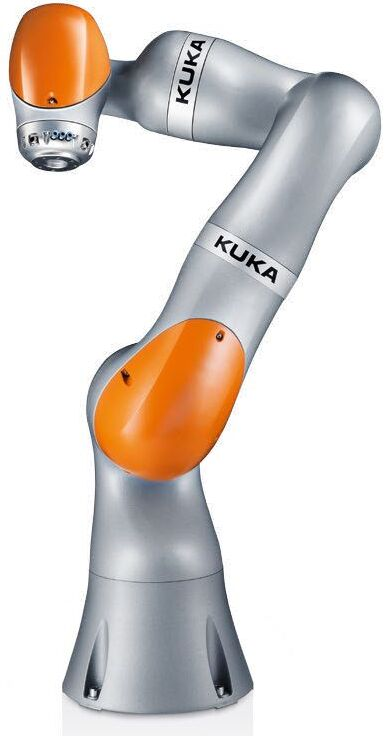
\includegraphics[width=5cm]{Imagem/KUKA.jpg}
    \caption{Robô KUKA LBR iiwa}
    \label{fig:robo_iiwa}
    \begin{flushleft}
    Fonte: \citeauthor{KUKAapresentacao}, p. 22, 2017b.
    \end{flushleft}
\end{figure}

O KUKA LBR iiwa está disponível no mercado em duas versões, com capacidades de carga útil de 7 kg e 14 kg e apresentam alcance máximo de 800 mm e 820 mm, respectivamente. Na FIG. \ref{fig:dimensoes} é possível verificar o espaço de trabalho e os parâmetros das dimensões do robô, enquanto na TAB. \ref{tab:dimensoes} é informado seus valores para ambos os modelos. Mais informações podem ser encontrada no Apêndice \ref{apend:dim}.

\begin{figure}[h]
    \centering
    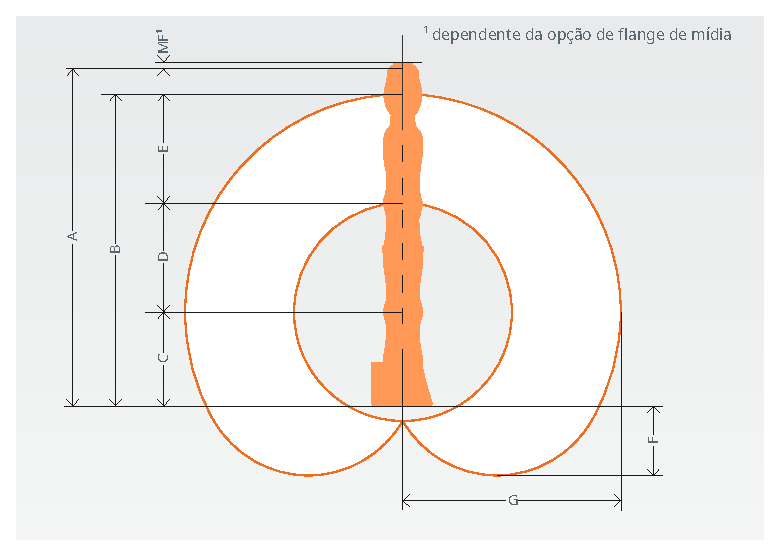
\includegraphics[width=0.48\textwidth]{Imagem/volume_trab.eps}
    \caption{Dimensões do KUKA LBR iiwa}
    \label{fig:dimensoes}
    \begin{flushleft}
    Fonte: KUKA, p. 30, 2017a. (Adaptação de     cores e tradução).
    \end{flushleft}
\end{figure}

\begin{table}[h]
    \centering
    \caption{Dimensões, em milímetros, dos parâmetros da FIG. \ref{fig:dimensoes}}
    \label{tab:dimensoes}
    \begin{tabular}{cccccccc}
    \toprule
        Robô & $A$ & $B$ & $C$ & $D$ & $E$ & $F$ & $G$ \\
    \midrule
         7 R800 & 1,266 & 1,140 & 340 & 400 & 400 & 260 & 800 \\
        14 R820 & 1,306 & 1,180 & 360 & 420 & 400 & 255 & 820 \\
    \bottomrule
    \end{tabular}
\end{table}

\subsection{Aplicações e Estudos de Casos}

Existem diversas áreas de aplicação em que o manipulador KUKA LBR é utilizado. Devido às suas características funcionais e sua adaptabilidade em trabalhar ao lado do fator humano, o robô é utilizado, principalmente, em indústrias de tecnologia e de produção em massa. As principais tarefas delegadas ao manipulador são aquelas de repetição monótona, como em funções de pintar, colar, aplicar, paletizar, embalar, medir e testar. Há também a utilização do robô na área de usinagem mecânica e montagem de peças.

% ANTES DA MODIFICAÇÃO Estudos de caso estão disponíveis no site da fabricante do robô, e vale ressaltar aqui, alguns em específico, como a solução desenvolvida pela KUKA para a montadora de veículos BMW, em uma de suas instalações localizada na cidade de Dingolfing na Alemanha.

Estudos de caso são apresentados na página web da fabricante do robô na qual algumas aplicações se destacam. Um exemplo é a solução desenvolvida pela fabricante KUKA para a montadora de veículos BMW em uma instalação localizada em Dingolfing, Alemanha. 

Em uma determinada etapa do processo de fabricação de veículos, os funcionários do Grupo BMW precisavam montar caixas de engrenagens de eixos dianteiros. Estes carregavam e levantavam peças de até 5 kg, de difícil acesso, com tolerâncias milimétricas de ajuste. A solução desenvolvida foi utilizar o robô KUKA LBR para montagem das engrenagens. O manipulador trabalha de forma suspensa e realiza o trabalho ``pesado'', poupando o esforço físico dos funcionários. 

%ANTES DA ALTERAÇÃO A garra foi projetada com revestimentos arredondados, protegendo os operadores de ferimentos. Além disso, sensores externos não são necessários, porque o LBR possui um sistema de sensor de torque articulado em cada um de seus sete eixos, fornecendo segurança aos operadores. (MUDEI PORQUE JÁ FALAMOS QUE TEM SENSOR DE TORQUE EM TODAS A JUNTAS, TENTEI AMENIZAR A REPETIÇÃO DA INFORMAÇÃO)

A garra foi projetada com revestimentos arredondados, protegendo assim os operadores de ferimentos. Além disso, sensores externos não são necessários devido à presença dos sensores de torque nas juntas que fornecem segurança aos operadores. Na FIG. \ref{fig:BMW} pode-se observar uma foto do robô operando na aplicação descrita. 

\begin{figure}[h]
    \centering
    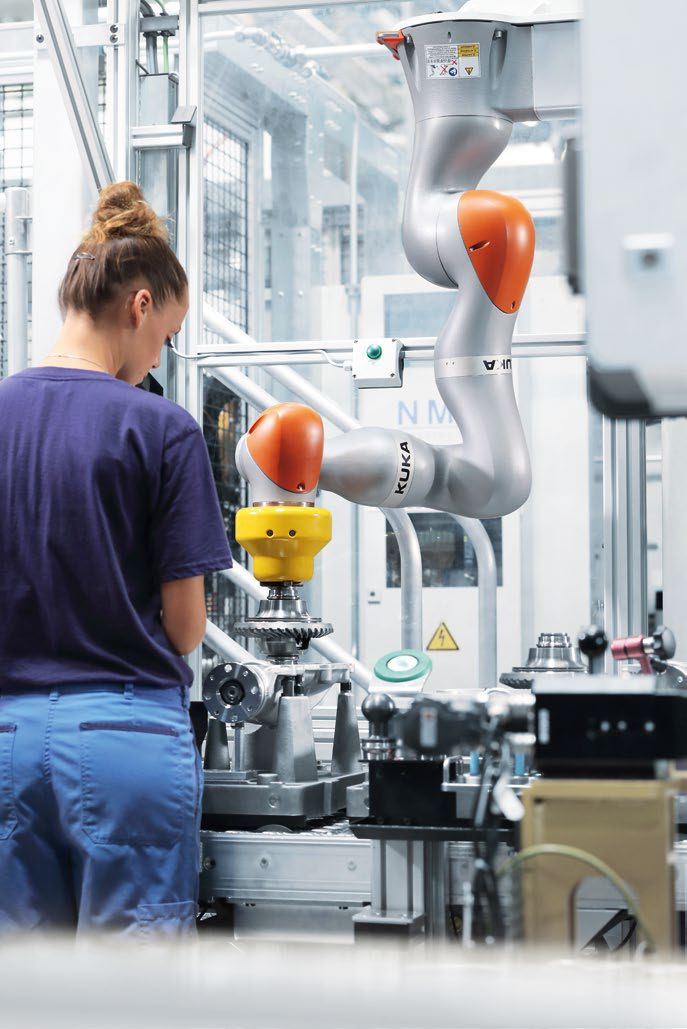
\includegraphics[width=0.48\textwidth]{Imagem/BMW.jpg}
    \caption{Instalação de peças em superfícies complexas de um monobloco da BMW}
    \label{fig:BMW}
    \begin{flushleft}
    Fonte: \citeauthor{KUKAmanual}, p. 28, \citeyear{KUKAmanual}.
    \end{flushleft}
\end{figure}

Outro estudo de caso a ser mencionado é a utilização do manipulador pela fabricante de equipamentos eletrônicos Siemens. No âmbito da fabricação de estatores a Siemens, na unidade de Bad Neustadt, também na Alemanha, procurava por uma solução flexível para automatizar a atividade simples de entrega e posicionamento de peças, que até então era feita manualmente. 

A solução criada foi o desenvolvimento de uma célula flexível com o robô de construção leve KUKA LBR iiwa. Assim, o robô, assume a função de retirar a peça a ser processada --– o estator composto de um corpo básico de chapa elétrica e placa de alumínio --- do porta-peças e encaminhá-la a um torno que fará a sua usinagem. Após este processo, o robô apanha as peças, faz uma limpeza por sopro e as destina à estação de medição.

\begin{figure}[h]
    \centering
    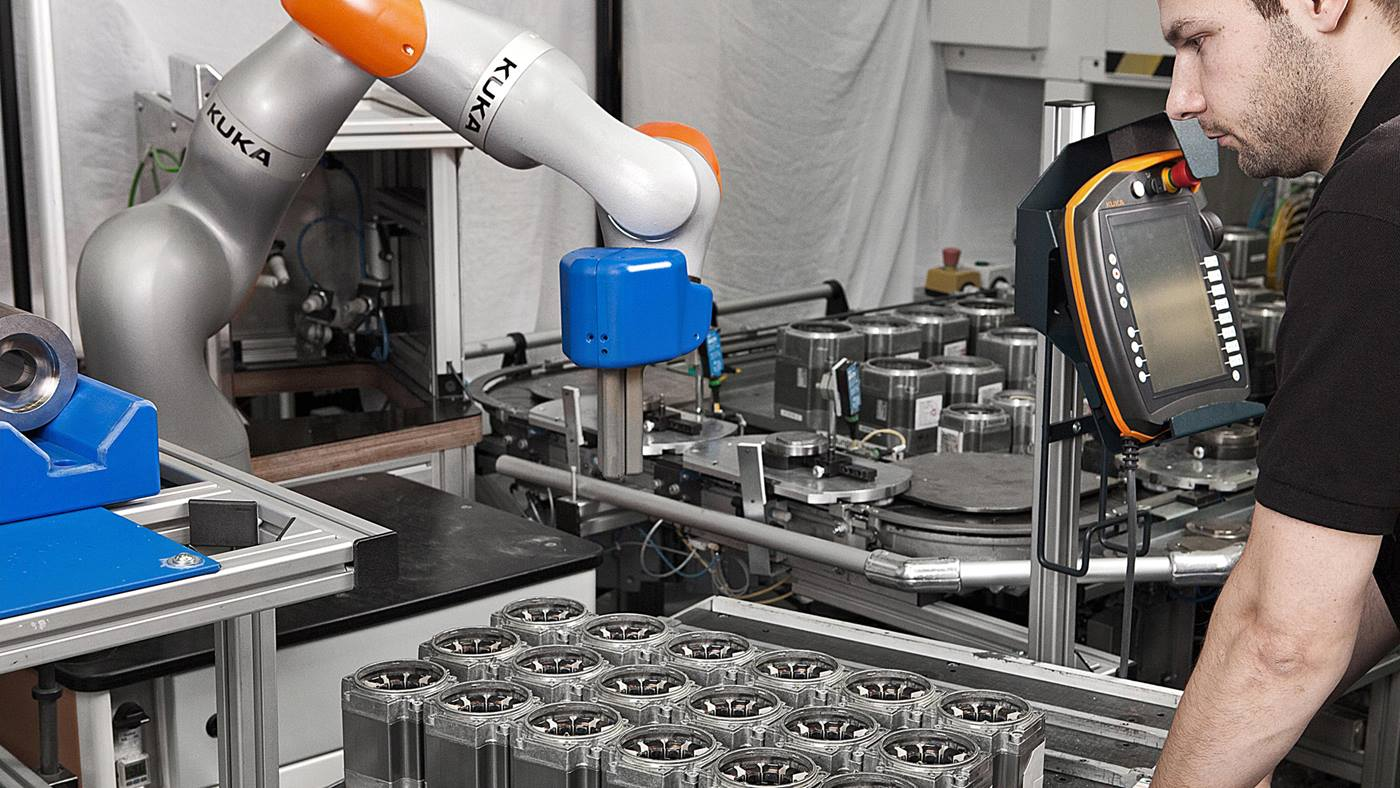
\includegraphics[width=8cm]{Imagem/Siemens.jpg}
    \caption{Carregamento automático de um torno CNC na Siemens}
    \label{fig:SIEMENS}
    \begin{flushleft}
    Fonte: \citeauthor{KUKAmanual}, p. 21, \citeyear{KUKAmanual}.
    \end{flushleft}
\end{figure}

Outros estudos de caso aos quais a implementação do robô simplificou os processos tecnológicos, são de empresas como a Ford, Volkswagen e Perschmann Calibration GmbH. 

Nas indústrias da Ford, vários robôs foram instalados para aplicar um cordão de vedação em diversas peças. Eles sempre aplicam o material exatamente na mesma posição e na quantidade definida. Assim é possível obter uma boa vedação na carroceria e evitar um retrabalho na pintura, eliminando custos.

Já na montadora alemã, Volkswagen, o robô KUKA LBR iiwa participa de processos de montagem, colagem e soldagem. Trabalhando ao lado do fator humano, o robô realiza suas funções com precisão e eficiência, como é mostrado na FIG \ref{fig:VW}. 

\begin{figure}[h]
    \centering
    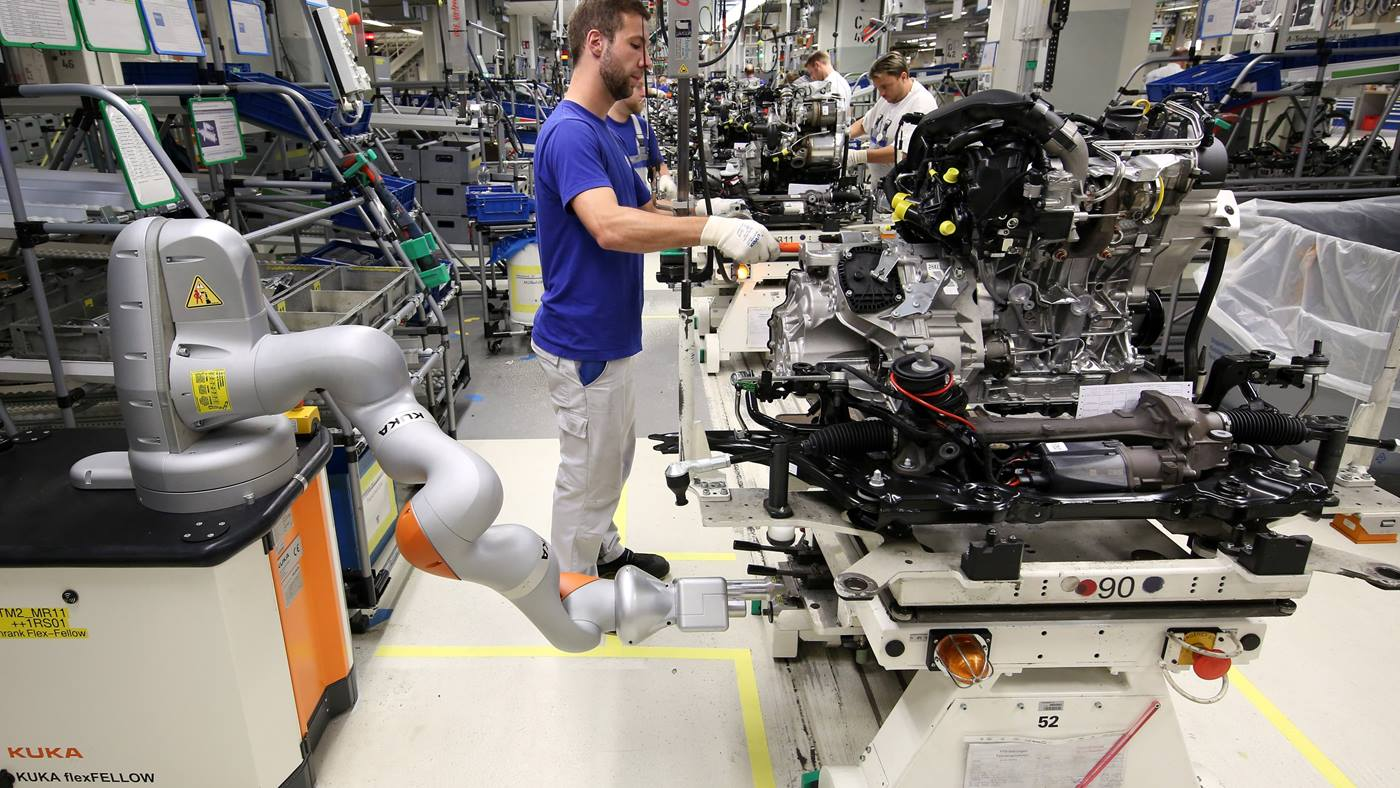
\includegraphics[width=8cm]{Imagem/VW.jpg}
    \caption{Montagem de peças na linha de produção}
    \label{fig:VW}
    \begin{flushleft}
    Fonte: \citeauthor{KUKAmanual}, p. 21, \citeyear{KUKAmanual}.
    \end{flushleft}
\end{figure}

A empresa  Perschmann Calibration GmbH, especialista em serviços de calibração, utiliza o manipulador como ferramenta de medição.  De acordo com o Dr. Detlef Rübesame, diretor Técnico da Perschmann Calibration, um cabelo humano tem aproximadamente \SI{50}{\micro\metre} de espessura, os fios de uma aranha, cerca de \SI{5}{\micro\metre}, e a precisão com a qual o robô faz sua calibração é de cerca de \SI{0,5}{\micro\metre}, um valor importante para manter a qualidade de seus serviços. Estes e outros estudos de caso endossam a importância do novo antropomorfo no mercado.

\section{Modelagem do Robô pelo método DH}
Existem diversas formas de se obter o modelo de um robô, tais como Denavit-Hartenberg clássico, Denavit-Hartenberg modificado e através das matrizes de transformação homogêneas de cada um dos \textit{frames} no robô. Nesse trabalho o método escolhido para se obter a expressão matemática foi Denavit-Hartenberg clássico. 

\subsection{Diagrama de arames}
O primeiro passo para a aplicação da técnica escolhida é fazer uma simplificação do manipulador robótico por meio da representação em diagrama de arames. Este deve ser feito com o robô em posição de \textit{home} conforme pode-se verificar na FIG. \ref{fig:home}.

\begin{figure}[h]
    \centering
    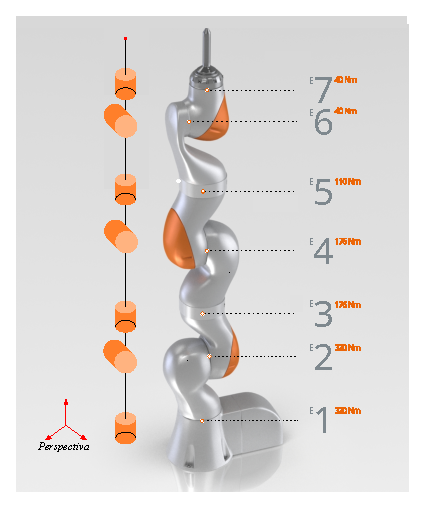
\includegraphics[width=0.45\textwidth]{Imagem/Arames.eps}
    \caption{Posição \textit{home} do manipulador.}
    \label{fig:home}
    Fonte: \citeauthor{KUKA3D}, 2020. (Desenho dos frames e indicação dos eixos e seus respectivos torques).
\end{figure}

\subsection{Atribuição de \ensuremath{z}}
Uma vez que o diagrama de arames foi definido então pode-se aplicar a convenção de Denavit-Hartenberg. Para determinar os frames do robô, deve-se atribuir os eixos $z_i$ nos eixos de atuação para cada junta $i+1$, sendo $i = 0,\;1,\;2,\dots,\;n-1$, em que $n$ é o número de juntas do manipulador. O eixo $z_n$, referente ao frame do \textit{end-effector} ou \textit{tool frame}, deve ser atribuído ao final. Após atribuir os eixos $z_i$, então pode-se identificar a origem dos frames $i$, em que $i=1,\;2,\;\dots,\;n-1$ adotando a seguinte regra: 

\begin{itemize}
    \item Se $z_{i-1}$ interceptar $z_i$, então a origem do frame $i$ deve ser posicionada na interseção.
    \item Se não, mas se existe uma perpendicular comum à $z_{i-1}$ e $z_i$, então a origem fica nessa reta perpendicular comum. 
    \item Se nenhuma das opções anteriores são verdadeiras, então $z_{i-1}$ e $z_i$ são paralelos e assim a origem do sistema de coordenadas deve ser posicionada de forma que o modelo fique mais simples. 
\end{itemize}

Para o robô aqui estudado, pôde-se adotar a primeira regra para todos os \textit{frames}. Isso porque $z_{i-1}$ e $z_i$ se interceptam para todo $i=1,\;2,\;\dots,\;n-1$.

\subsection{Atribuição de \ensuremath{x}}
Com as origens $o_i$ e os eixos $z_i$ determinados, estabelece-se os eixos $x_i$, para $i=1,\;2,\;\dots,\;n-1$, considerando a seguinte regra:

\begin{itemize}
    \item Se $z_{i-1}$ interceptar $z_i$, então $x_i$ deve ser posicionado na direção normal ao plano de $z_{i-1}$e $z_i$
    \item Se não, então determina-se $x_i$ na perpendicular comum de $z_{i-1}$e $z_i$ a partir da origem do \textit{frame} $i$.  
\end{itemize}

No KUKA LBR iiwa, para todo $i=1,\;2,\;\dots,\;n-1$, os eixos $x_i$ foram atribuídos conforme a primeira regra.

\subsection{Atribuição de \ensuremath{y}}
Os eixos $y_i$ foram escolhidos implicitamente de forma que todos os sistemas de coordenadas fossem dextrogiros, como requerido pelo método clássico de Denavit-Hartenberg. Portanto, optou-se por excluí-lo do diagrama da FIG. \ref{fig:frames} para deixar mais fácil a sua visualização e obtenção dos parâmetros dos links.

\subsection{Referência e End-effector}
Por fim, foram atribuídos os \textit{frames} $0$ e $n$. Para o \textbf{end-effector}, já que o robô não apresenta garra, repetiu-se o frame $6$, como instruído no método DH clássico. O \textit{frame} $i=0$ foi atribuído na base do robô. Embora a atribuição não seja a mais simples, visto que se sua origem fosse atribuída junto aos \textit{frames} 1 e 2 reduzir-se-ia uma translação, ela facilitará na comparação dos resultados com a simulação no RoboDK. A FIG. \ref{fig:frames} expõe a atribuição de \textit{frames} descrita.

\begin{figure}[ht]
    \centering
    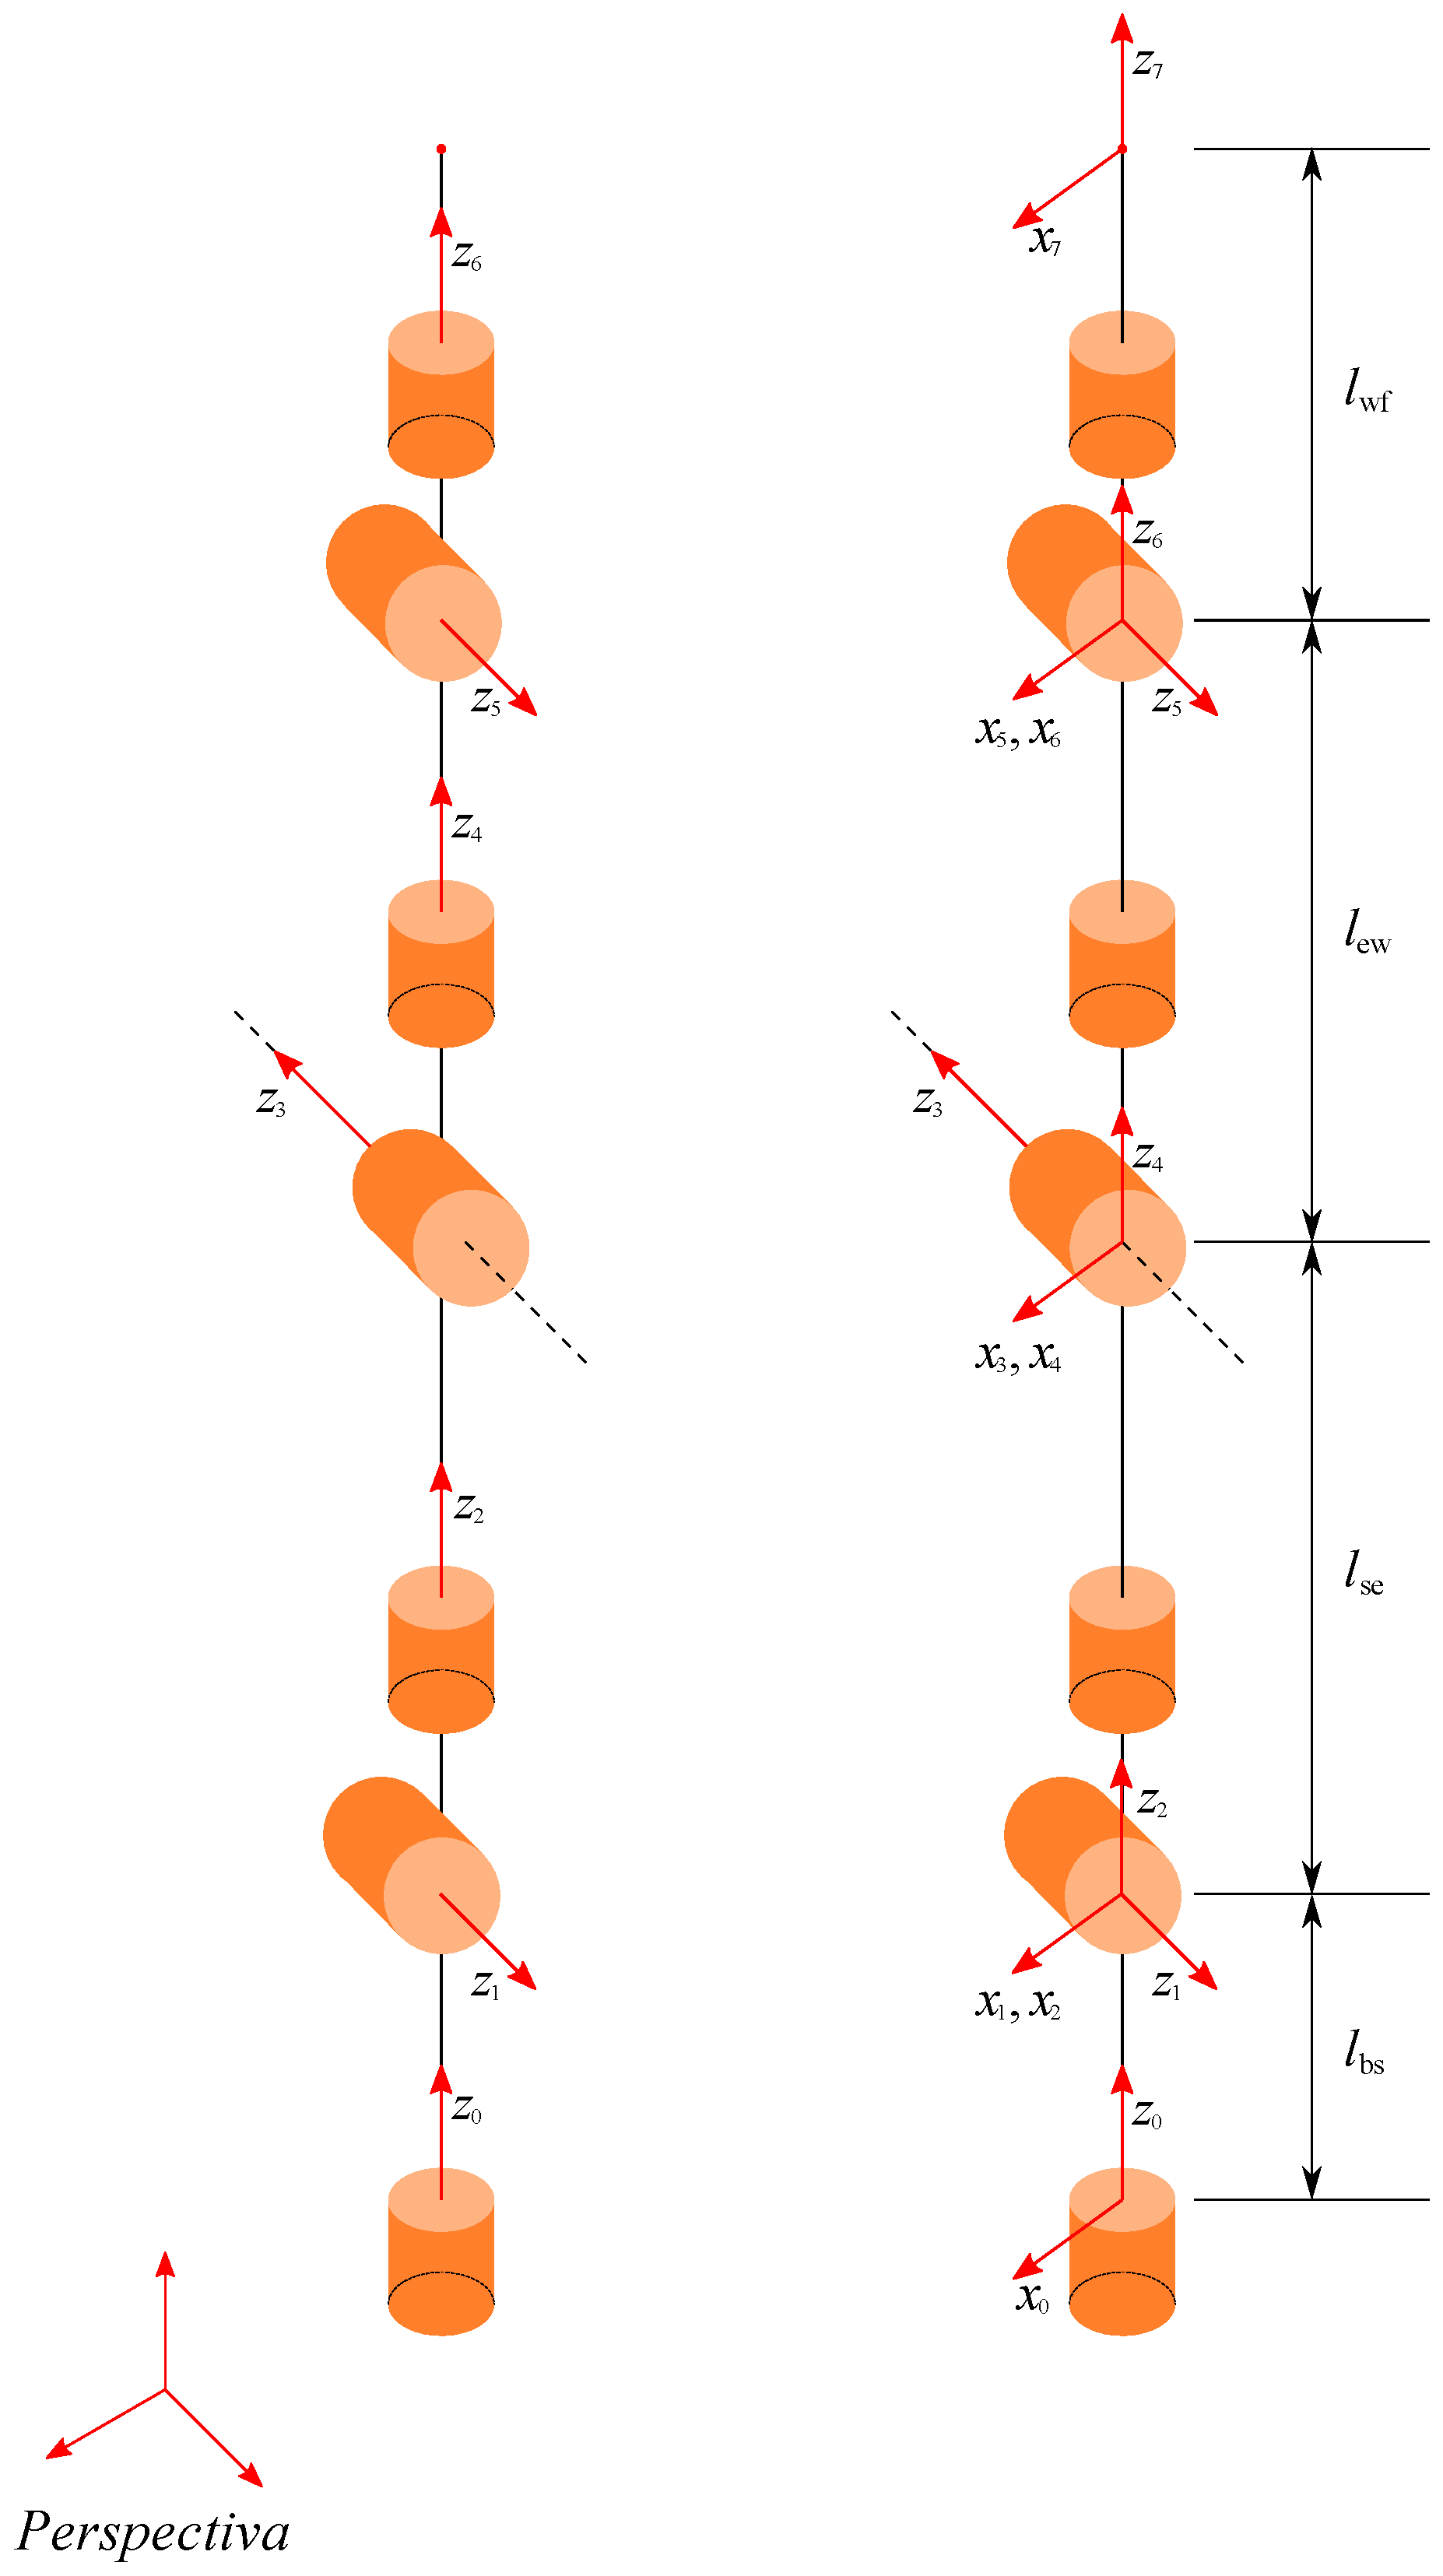
\includegraphics[width=0.45\textwidth]{Imagem/x.eps}
    \caption{Atribuição dos \textit{frames}}
    \label{fig:frames}
\end{figure}

\subsection{Tabela de Denavit-Hartenberg}

Após dispor todos os \textit{frames}, são determinados os parâmetros da tabela de Denavit-Hartenberg. Em cada uma de suas linhas é possível definir a matriz de transformação homogênea $A_i$ do \textit{frame} $i-1$ para o \textit{frame} $i$, fazendo  
\begin{align*}
  \setlength{\dashlinegap}{2pt}
    A_i
    &= \Rot_{z,\,\theta_i} \Trans_{z,\,d_i} \Trans_{x,\,a_i} \Rot_{x,\,\alpha_i} \\
    &=
    \left[ 
    \begin{array}{rrr;{2pt/2pt}c}
        c_{\theta_i} & -s_{\theta_i}c_{\alpha_i} & s_{\theta_i} s_{\alpha_i} & a_i c_{\theta_i} \\
        s_{\theta_i} & c_{\theta_i} c_{\alpha} & -c_{\theta_i} s_{\alpha} & a_i s_{\theta_i} \\
        0 & s_{\alpha_i} & c_{\alpha_i} & d_i \\
        \hdashline[2pt/2pt]
        0 & 0 & 0 & 1
    \end{array}
    \right]
\end{align*}
em que $a_i$ é a distância entre $z_{i-1}$ e $z_i$ medido ao longo de $x_i$; $\alpha_i$ o ângulo entre $z_{i-1}$ e $z_i$ mensurado no plano normal a $x_i$;  $d_i$ a distância perpendicular entre a origem $o_{i-1}$ e a interseção de $x_i$ com $z_{i-1}$, medido ao longo de $z_0$; $\theta_i$ o ângulo  entre $x_0$ e $x_1$ mensurado no plano normal a $z_0$.

Uma vez obtidas as matrizes $A_i$ para $i= 1,\;2,\;\dots,\;n$, então pode-se determinar a matriz de transformação $T$ do \textit{frame} $0$ para o \textit{frame} $n$ como
\begin{equation*}
    T_n^0 = \prod_{i=0}^n A_i
\end{equation*}

Para o braço robótico KUKA LBR iiwa, os parâmetros da tabela DH podem ser retirados da sua interpretação física da atribuição de \textit{frames} vista na FIG. \ref{fig:frames}. A TAB. \ref{tab:DH} expõe os valores obtidos. 

\begin{table}[h]
    \centering
    \caption{Parâmetros DH do KUKA LBR iiwa}
    \label{tab:DH}
    \begin{tabular}{crrrr}
    \toprule
        $i$ & $a_i$ & $\alpha_i$ & $d_i$ & $\theta_i$ \\
    \midrule
        1 & 0 & $-\pi/2$ & $\ell_\mathrm{bs}$ & $\theta_1^*$ \\
        2 & 0 &  $\pi/2$ &                  0 & $\theta_2^*$ \\
        3 & 0 &  $\pi/2$ & $\ell_\mathrm{se}$ & $\theta_3^*$ \\
        4 & 0 & $-\pi/2$ &                  0 & $\theta_4^*$ \\
        5 & 0 & $-\pi/2$ & $\ell_\mathrm{ew}$ & $\theta_5^*$ \\
        6 & 0 &  $\pi/2$ &                  0 & $\theta_6^*$ \\
        7 & 0 &        0 & $\ell_\mathrm{wf}$ & $\theta_7^*$ \\
    \bottomrule
    \end{tabular}
    
O $^*$ indica que é variável.
\end{table}

Para o link 1, segue $a_1 = 0$, $\alpha_1 = -\pi/2$, $d_1=\ell_\mathrm{bs}$ e $\theta_1$ sendo a variável, então
\begin{align*}
    A_1 
    &=
    \left[ 
    \begin{array}{rrr;{2pt/2pt}c}
        c_{\theta_1} & 0 & -s_{\theta_1} & 0 \\
        s_{\theta_1} & 0 &  c_{\theta_1} & 0 \\
        0 & -1 & 0 & \ell_\mathrm{bs} \\
        \hdashline[2pt/2pt]
        0 & 0 & 0 & 1
    \end{array}
    \right]
\end{align*}
Para o link 2, segue $a_2 = 0$, $\alpha_2 = \pi/2$, $d_2=0$ e $\theta_2$ sendo a variável, então
\begin{align*}
    A_2 &=
    \left[ 
    \begin{array}{rrr;{2pt/2pt}c}
        c_{\theta_2} & 0 &  s_{\theta_2} & 0 \\
        s_{\theta_2} & 0 & -c_{\theta_2} & 0 \\
        0 & 1 & 0 &  0 \\
        \hdashline[2pt/2pt]
        0 & 0 & 0 & 1
    \end{array}
    \right]
\end{align*}
Para o link 3, segue $a_3 = 0$, $\alpha_3 = \pi/2$, $d_3=\ell_\mathrm{se}$ e $\theta_3$ sendo a variável, então
\begin{align*}
    A_3 &=
    \left[ 
    \begin{array}{rrr;{2pt/2pt}c}
        c_{\theta_3} & 0 &  s_{\theta_3} & 0 \\
        s_{\theta_3} & 0 & -c_{\theta_3} & 0 \\
        0 & 1 & 0 &  \ell_\mathrm{se} \\
        \hdashline[2pt/2pt]
        0 & 0 & 0 & 1
    \end{array}
    \right]
\end{align*}
Para o link 4, segue $a_4 = 0$, $\alpha_4 = -\pi/2$, $d_4=0$ e $\theta_4$ sendo a variável, então
\begin{align*}
    A_4 
    &=
    \left[ 
    \begin{array}{rrr;{2pt/2pt}c}
        c_{\theta_4} & 0 & -s_{\theta_4} & 0 \\
        s_{\theta_4} & 0 &  c_{\theta_4} & 0 \\
        0 & -1 & 0 & 0 \\
        \hdashline[2pt/2pt]
        0 & 0 & 0 & 1
    \end{array}
    \right]
\end{align*}

Para o link 5, segue $a_5 = 0$, $\alpha_5 = -\pi/2$, $d_5=\ell_\mathrm{ew}$ e $\theta_5$ sendo a variável, então
\begin{align*}
    A_5 &=
    \left[ 
    \begin{array}{rrr;{2pt/2pt}c}
        c_{\theta_5} & 0 & -s_{\theta_5} & 0 \\
        s_{\theta_5} & 0 &  c_{\theta_5} & 0 \\
        0 & -1 & 0 &  \ell_\mathrm{ew} \\
        \hdashline[2pt/2pt]
        0 & 0 & 0 & 1
    \end{array}
    \right]
\end{align*}
Para o link 6, segue $a_6 = 0$, $\alpha_6 = \pi/2$, $d_6=0$ e $\theta_6$ sendo a variável, então
\begin{align*}
    A_6 &=
    \left[ 
    \begin{array}{rrr;{2pt/2pt}c}
        c_{\theta_6} & 0 &  s_{\theta_6} & 0 \\
        s_{\theta_6} & 0 & -c_{\theta_6} & 0 \\
        0 & 1 & 0 &  0 \\
        \hdashline[2pt/2pt]
        0 & 0 & 0 & 1
    \end{array}
    \right]
\end{align*}
Para o link 7, $a_7 = 0$, $\alpha_7 = 0$, $d_7=\ell_\mathrm{wf}$ e sendo $\theta_7$ a variável, segue
    \begin{align*}
        A_7 =
        \left[ 
    \begin{array}{rrr;{2pt/2pt}c}
        c_{\theta_7} & -s_{\theta_7} & 0 & 0 \\
        s_{\theta_7} &  c_{\theta_7} & 0 & 0 \\
        0 & 0 & 1 & \ell_\mathrm{wf} \\
        \hdashline[2pt/2pt]
        0 & 0 & 0 & 1
    \end{array}
    \right]
    \end{align*}
    Por fim, a matriz de transformação homogênea do \textit{frame} 7 para o \textit{frame} 0 é encontrada fazendo
    \begin{equation}
        T_7^0 = A_1 A_2 A_3 A_4 A_5 A_6 A_7
    \end{equation}
uma multiplicação de 7 matrizes $4\times4$ de variáveis reais. A solução dessa multiplicação, matriz de transformação $T_7^0$, pode ser verificada no Apêndice \ref{apend:MatrizT}, para qual foram adotadas as dimensões do KUKA LBR iiwa 14 820
\begin{alignat*}{3}
\ell_\mathrm{bs} &= \SI{360}{mm}, \quad& \ell_\mathrm{se} &= \SI{420}{mm}, \\
\ell_\mathrm{ew} &= \SI{400}{mm}, \quad & \ell_\mathrm{wf} &= \SI{90}{mm}.
\end{alignat*}

A matriz foi obtida via simulação computacional, realizada por meio de um código em \texttt{Python 3}, exposto no Apêndice \ref{apend:memoria_calculo}.
\section{Validação do Modelo}
%Tendo encontrado o modelo cinemático, representado por $T_7^0$, é importante realizar sua validação. Isso pode ser feito através de análise dimensional ou por simulação computacional. No primeiro caso o modelo é aplicado à duas situações de conjuntos de valores das variáveis de juntas, sendo gerado a pose do \textit{end-effector}. Com isto, é comparado os resultados da matriz de transformação com o comportamento esperado.

%Para verificar a coerência do modelo obtido com o robô real foram escolhidas as condições de posição inicial de todos os ângulos em zero (conhecida como \textit{home}) e uma segunda condição para os ângulos $\theta_4 = -\pi/2$ e $\theta_5 = \pi/3$, mantendo os demais ângulos em zero. Assim foram obtidas as matrizes $T_\mathrm{home}$ e $T_\mathrm{escolhido}$, respectivamente.


Tendo encontrado o modelo cinemático, representado por $T_7^0$, é importante realizar sua validação. Isto é, verificar a coerência entre a representação matemática e o robô real. Isso pode ser feito através de análise dimensional ou por simulação computacional. No primeiro caso, é aplicado ao modelo um conjunto de valores de entrada, ou seja, são aplicados na matriz $T_7^0$ um conjunto de valores para os ângulos das juntas. Assim, obtém-se uma matriz que representa a pose do \textit{end-effector} em relação ao \textit{frame} 0 que deve corresponder ao diagrama de arames desenhado para a entrada de dados aplicada ao modelo. É recomendado que esse procedimento seja feito para duas entradas diferentes.

Nesse trabalho aplicou-se um conjunto de ângulos que representam a posição \textit{home}, $\theta_i=0$ para $i= 1, ... , 7$ e outro conjunto para uma posição escolhida dada por $\theta_1=\theta_2=\theta_3=\theta_6=\theta_7=0$, $\theta_4 = -\pi/2$ e $\theta_5 = \pi/3$. Assim, aplicando os ângulos das juntas nas equações apresentadas no Apêndice \ref{apend:MatrizT}, foram obtidas as matrizes
\begin{align}
T_\mathrm{home}
    &=
    \left[ 
    \begin{array}{rrr;{2pt/2pt}c}
        1 & 0 &  0 & 0 \\
        0 & 1 & 0 & 0 \\
        0 & 0 & 1 & 1270 \\
        \hdashline[2pt/2pt]
        0 & 0 & 0 & 1
    \end{array}
    \right],
    \label{eq:Thome} \\
T_\mathrm{escolhido}
    &=
    \left[ 
    \begin{array}{rrr;{2pt/2pt}c}
        0 & 0 & 1 & 490 \\
        \frac{\sqrt{3}}{2} & \frac{1}{2} &  0 & 0 \\
        -\frac{1}{2} & \frac{\sqrt{3}}{2} & 0 & 780 \\
        \hdashline[2pt/2pt]
        0 & 0 & 0 & 1
    \end{array}
    \right].
    \label{eq:Tescolhido}
\end{align}

A matriz $T_\mathrm{home}$ confirma as duas características da pose do robô em \textit{home}. A primeira é a translação que se concentra apenas no eixo $z$ cujo valor é a soma das extensões de todos os links. A segunda característica se refere à rotação, a qual percebe-se ser de valor zero nos três eixos devido à matriz de rotação estar expressa como uma matriz identidade. A representação em diagrama de arames desta condição confirma as características supracitadas e pode ser visto na FIG. \ref{diagramahome}.
\begin{figure}[h]
    \centering
    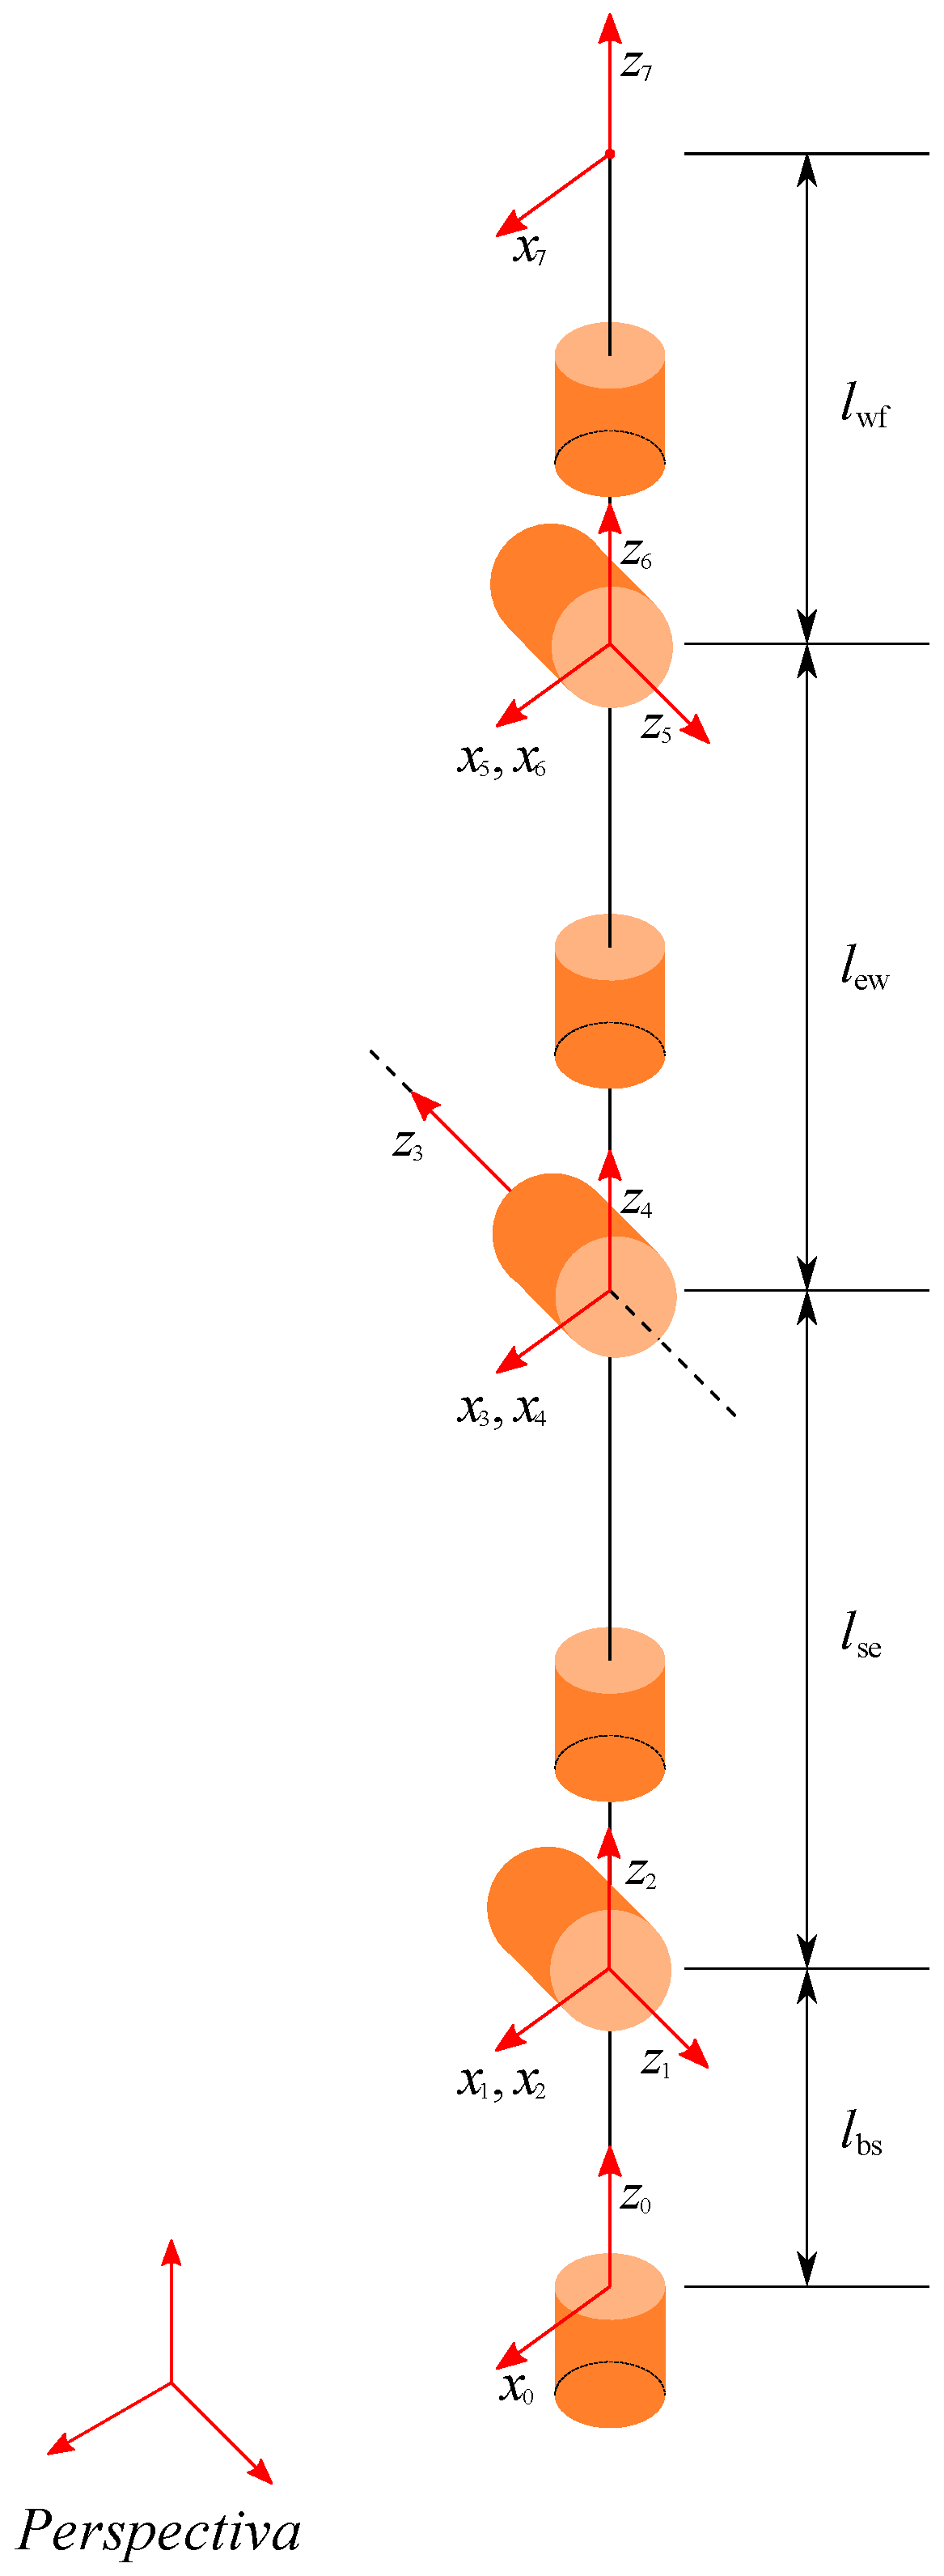
\includegraphics[width=3.5cm]{Imagem/validacao_home.eps}
    \caption{Diagrama esquemático da posição home}
    \label{diagramahome}
\end{figure}

Já para a matriz $T_\mathrm{escolhida}$, tem-se rotação de $-\ang{90}$ em $\theta_4$, o que distribui as translações nos eixos $z_0$, com valor de 780 mm representando a soma dos links $bs$ e $se$ ou do \textit{frame} zero ao quatro, e o restante da extensão do robô, 490 mm, fica direcionado paralelamente ao eixo $x_0$.

Após a curvatura de $-\ang{90}$ em $\theta_4$, tem-se a rotação do link 5 que faz com que o restante do braço do robô rotacione. O \textit{frame} final se dá portanto pelo resultado de uma composição de duas rotações e das translações relacionadas acima relação ao \textit{frame} zero.

O diagrama de arames mostrado na FIG. \ref{fig:condicaoescolhida} mostra os passos tomados para a avaliação desta nova pose. Em (a) o frame 4 é rotacionado em $-\ang{90}$; em (b) é feita a composição total do robô para tal rotação. Para (c) é mostrada a rotação do eixo 5 devido a rotação em $\theta_5$ e (d) é mostrado a configuração final do robô.

\begin{figure}[h]
    \centering
    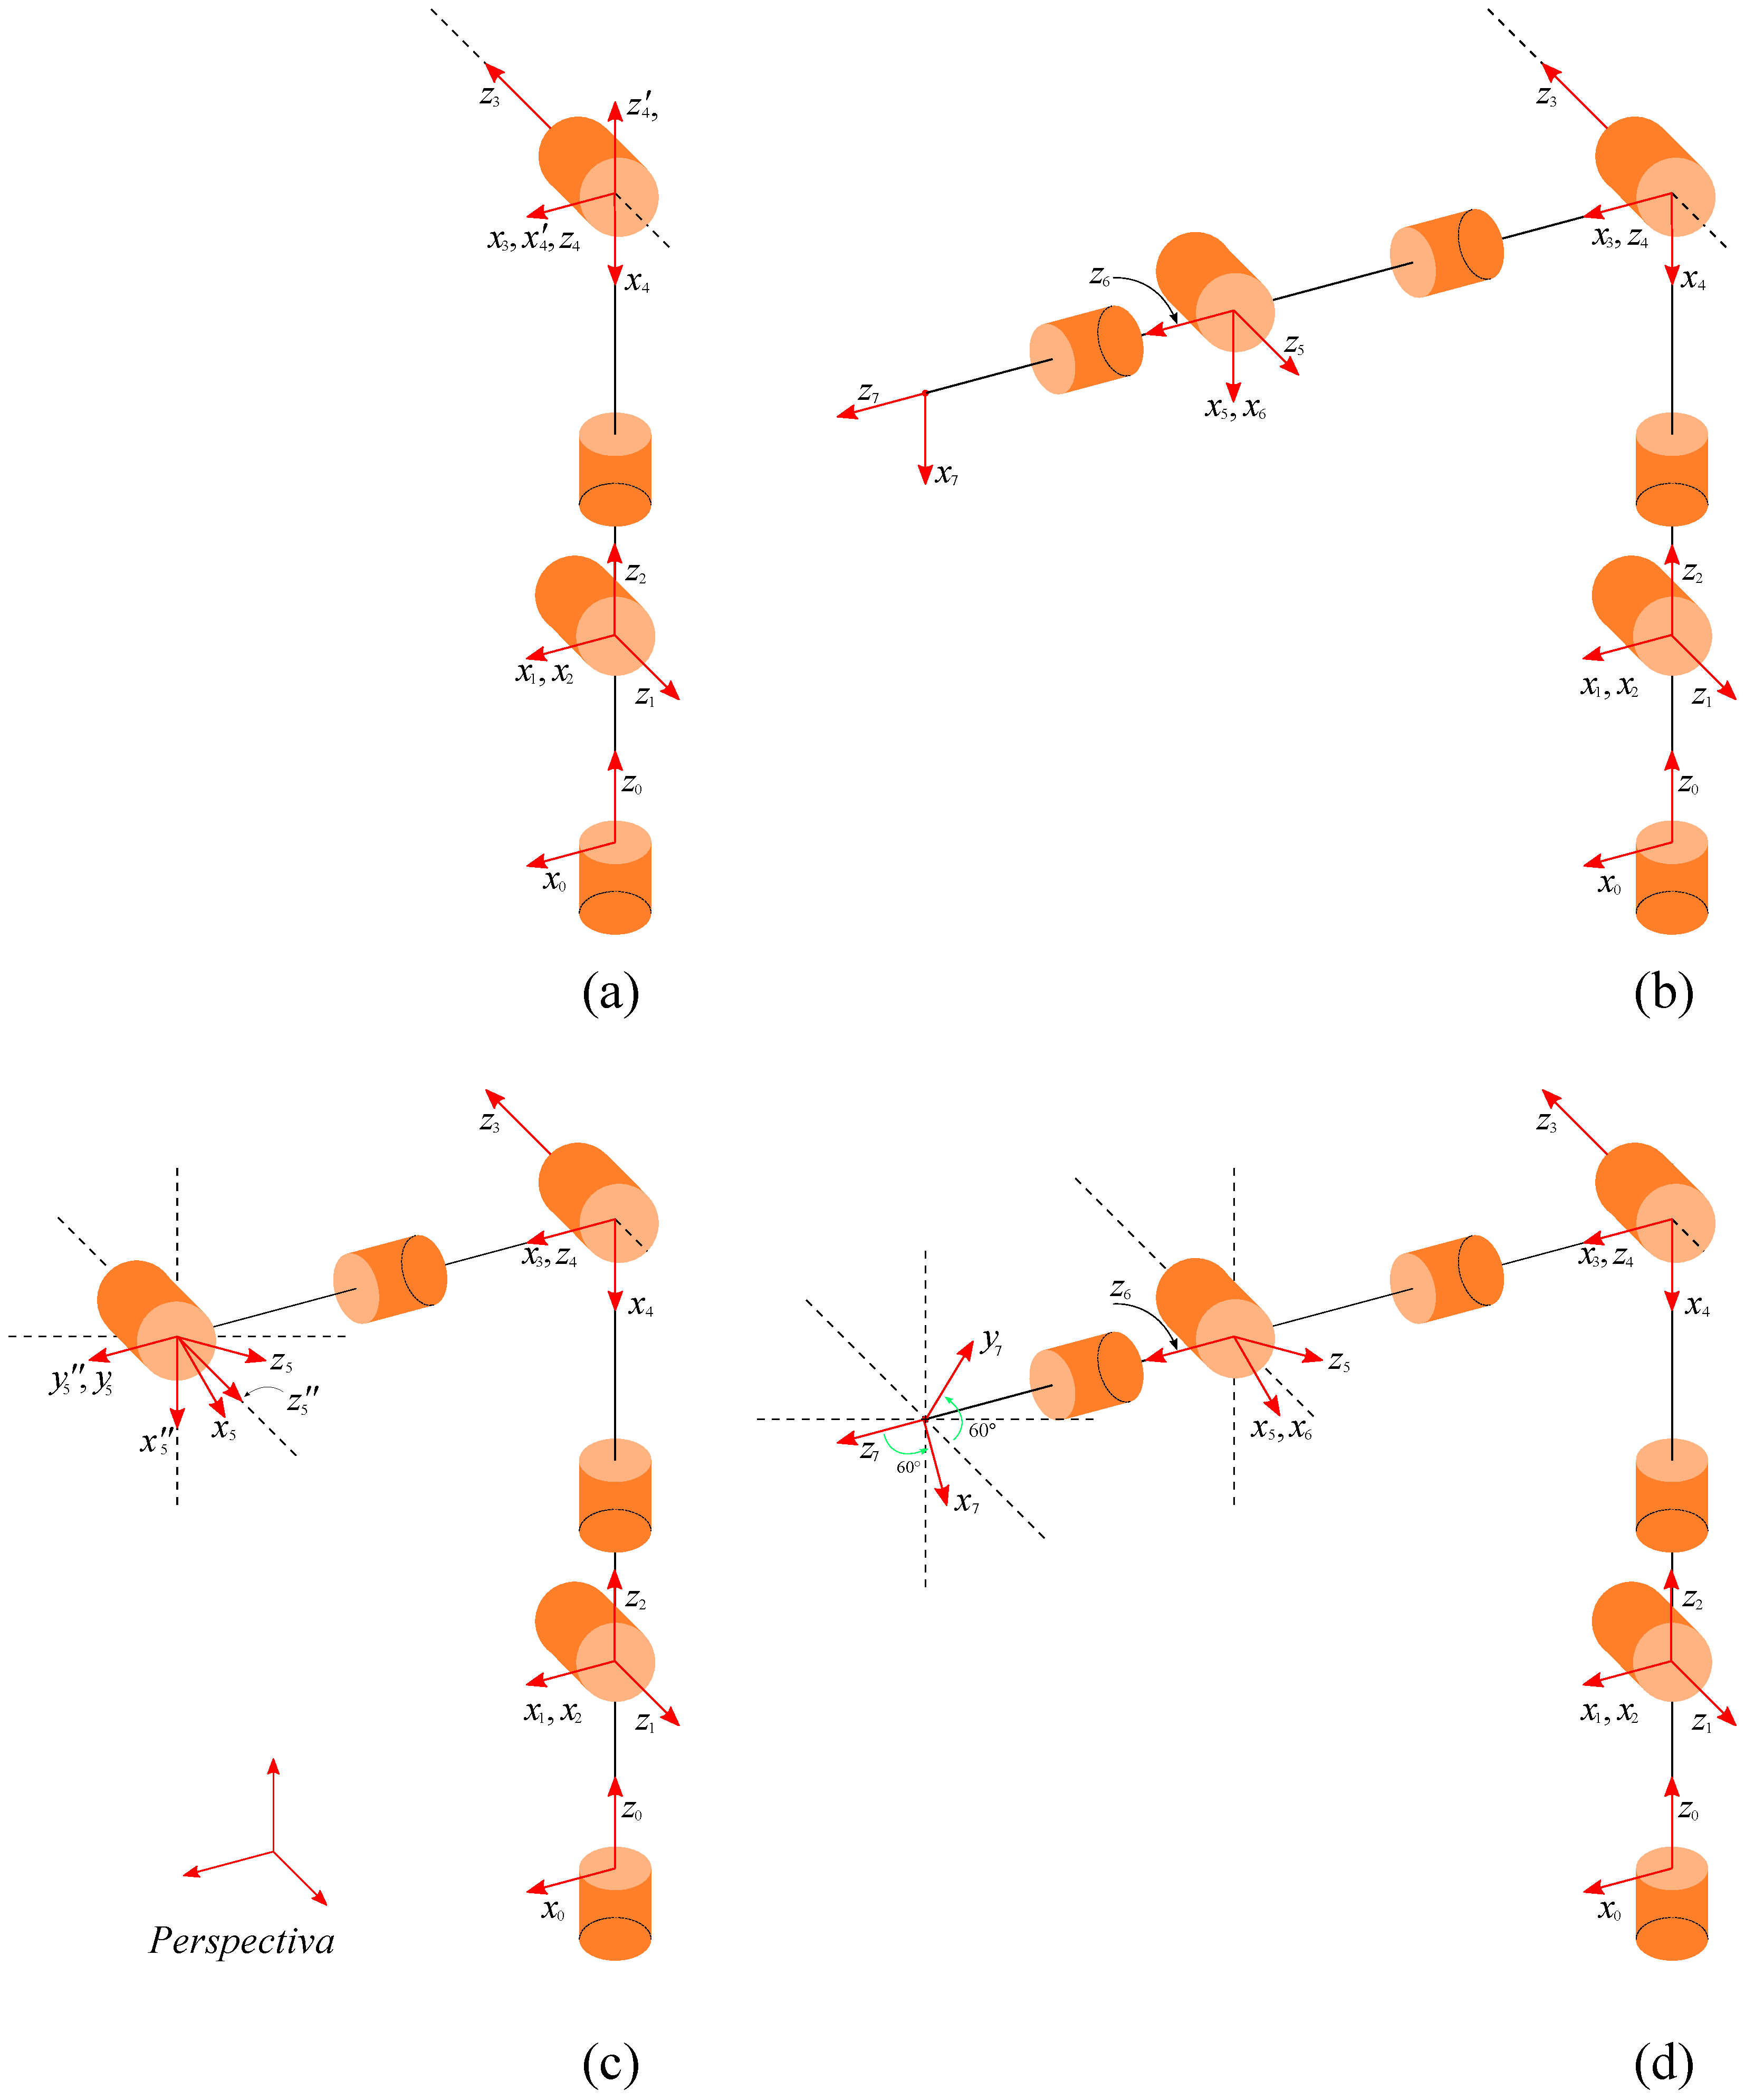
\includegraphics[width=8cm]{Imagem/validacao.eps}
    \caption{Passo-a-passo da representação esquemática da posição escolhida}
    \label{fig:condicaoescolhida}
\end{figure}

Note que a rotação do \textit{end-effector} pode ser analisando resolvendo
\begin{equation}
    R_7^0 = \Big[ x_7^0 \:\big|\: y_7^0 \:\big|\: z_7^0 \Big] = \left[\begin{array}{ccccc}
        x_7 \cdot x_0 && y_7 \cdot x_0 && z_7 \cdot x_0 \\
        x_7 \cdot y_0 && y_7 \cdot y_0 && z_7 \cdot y_0 \\
        x_7 \cdot z_0 && y_7 \cdot z_0 && z_7 \cdot z_0
    \end{array}\right]
    \label{eq:matrizR_generica}
\end{equation}

Na FIG. \ref{fig:zoom_pose_escolhido} nota-se inicialmente que $z_7 \cdot x_0 = 1$ então $x_7 \cdot x_0 = 0$, $y_7 \cdot x_0 = 0$, $z_7 \cdot y_0 = 0$ e $z_7 \cdot z_0 = 0$, visto que a matriz de rotação é ortonormal.
\begin{figure}[h]
    \centering
    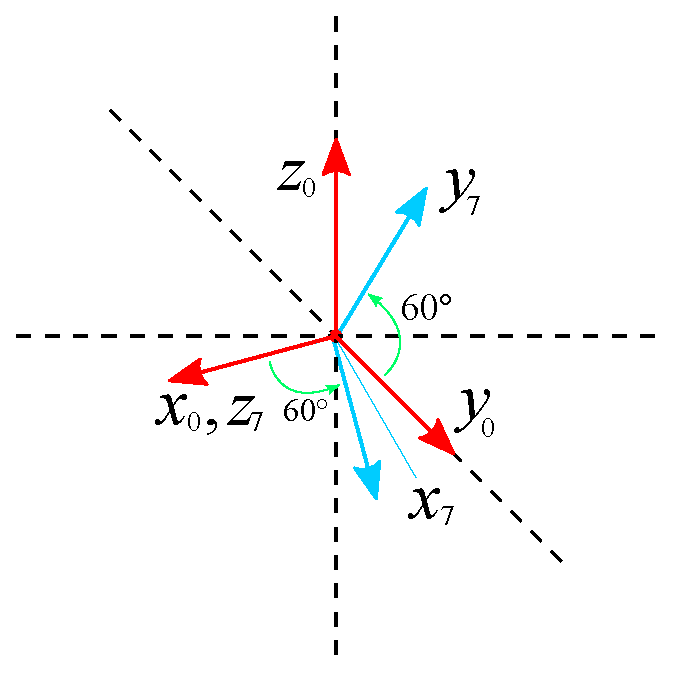
\includegraphics[width=5cm]{Imagem/zoom_pos-escolhida.eps}
    \caption{Orientação do \textit{end-effector}}
    \label{fig:zoom_pose_escolhido}
\end{figure}

Fazendo a projeção de $x_7$ em $y_0$ segue $\sen \ang{60} = \sqrt{3}/2$. Para $x_7$ em $z_0$, temos $-\cos \ang{60}$. Ainda, repetindo o processo para $y_7$, chega-se a $y_7 \cdot y_0 = \cos \ang{60}$ e $y_7 \cdot z_0 = \sen \ang{60}$. Portanto, a matriz que representa a orientação do \textit{frame} 7 é
\begin{equation}
    R_7^0 = \left[\begin{array}{rrrrr}
        0 && 0 && 1 \\
         \sqrt{3}/2 && 1/2 && 0 \\
        -1/2 && \sqrt{3}/2 && 0
    \end{array}\right]
    \label{eq:R_validacao}
\end{equation}

Comparando \eqref{eq:Tescolhido} com \eqref{eq:R_validacao}, verifica-se que a orientação da matriz de transformação é como se esperava. Destarte, o modelo cinemático do robô KUKA iiwa obtido foi validado.

\section{Simulação}
A simulação foi realizada no software RoboDK, software offline utilizado para simulação de robôs industriais. Para realização da simulação foram utilizados as posições escolhidas na análise dimensional. Ao se comparar os resultados de $T_\mathrm{home}$ e $T_\mathrm{escolhido}$, é possível comprovar que a matriz T representa o modelo cinemático do robô.

Para comprovar o explicito acima, inicialmente, analisa-se a posição do modelo em \textit{home}, como indicado na FIG. \ref{fig:home_simulacao}.

\begin{figure}[ht]
    \centering
    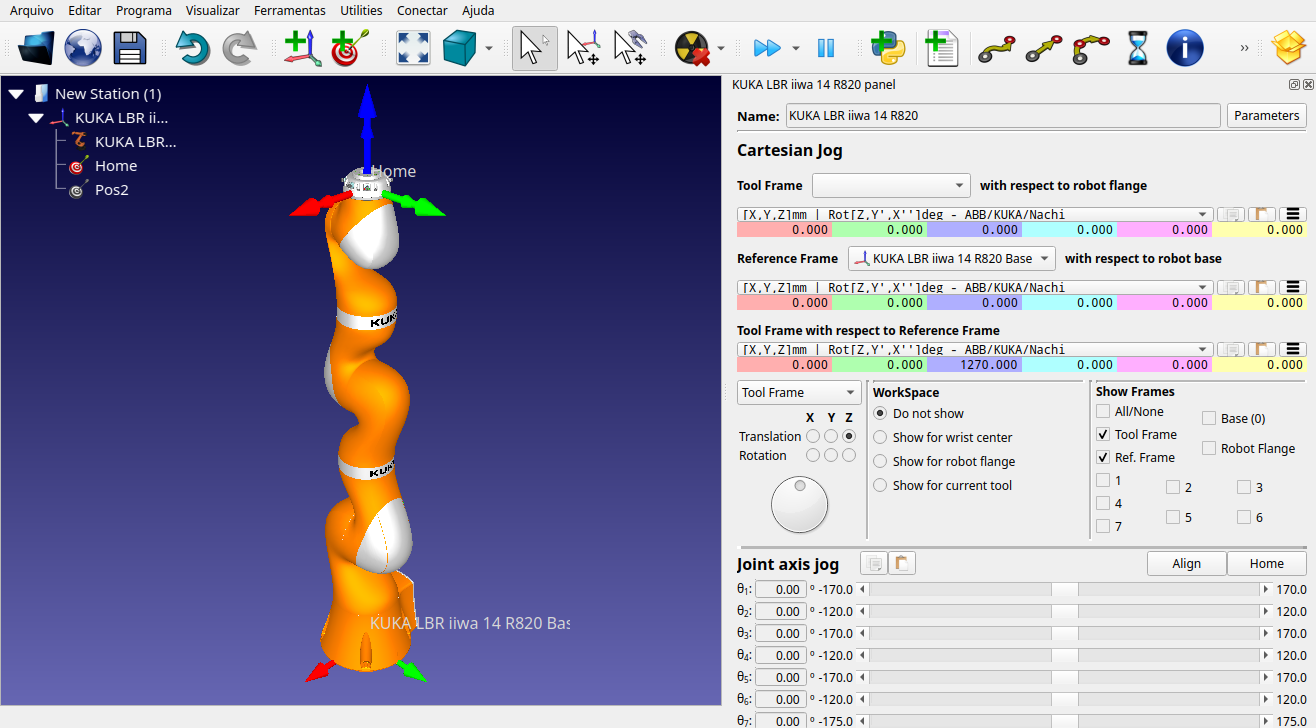
\includegraphics[scale=0.25]{Imagem/home.png}
    \caption{Posição home do robô KUKA LBR iiwa}
    \label{fig:home_simulacao}
\end{figure}

A análise da FIG. \ref{fig:home_simulacao} indica que, inicialmente, não há rotações do frame zero para o frame final, porém existe um único deslocamento no eixo $z_{0}$ correspondente ao valor total da soma dos links, sendo este de 127 cm. 

na condição seguinte, o robô foi foi simulado para a posição escolhida, como indicado na FIG. \ref{fig:escolhida}.

\begin{figure}[h]
    \centering
    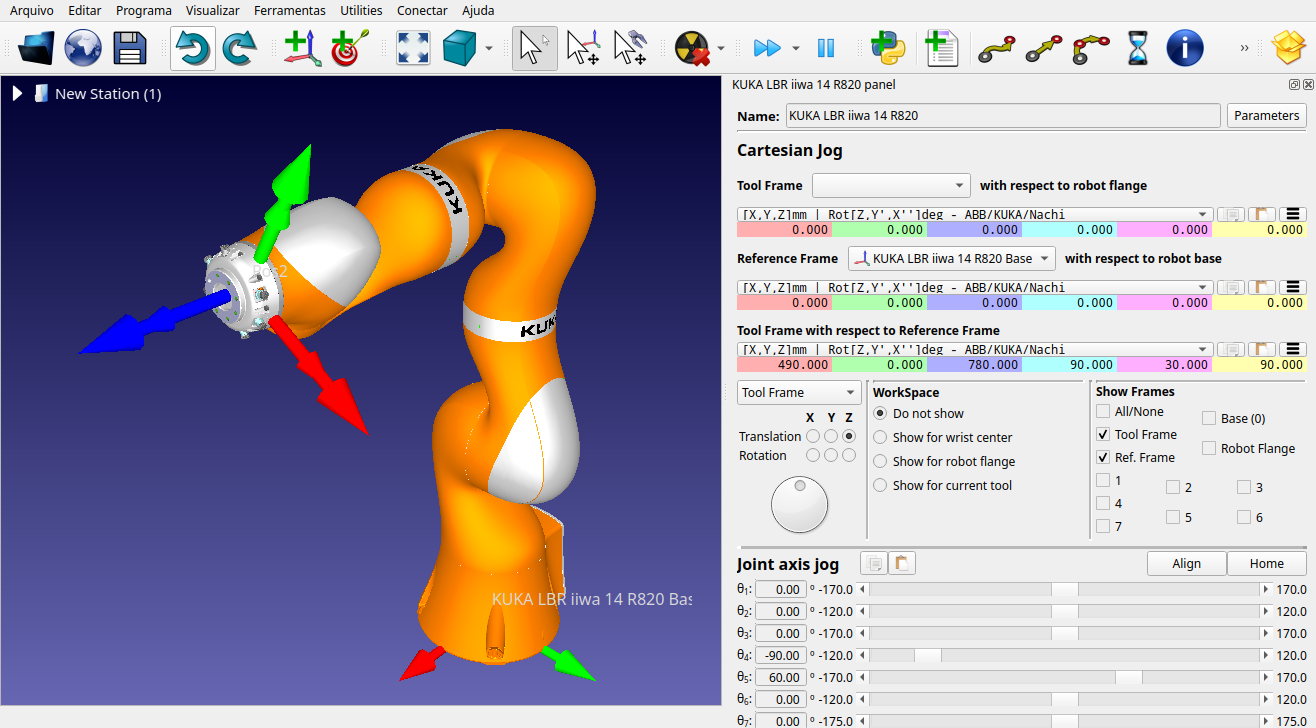
\includegraphics[width=8cm]{Imagem/escolhido.png}
    \caption{Posição escolhida para o robô KUKA LBR iiwa}
    \label{fig:escolhida}
\end{figure}

É possível observar que, do frame zero ao quatro tem-se um a translação de  da pose \textit{home} para a escolhida, ocorreu uma rotação de \ang{60} no link 5 ($\theta_5$) e de $-\ang{90}$ no link 4 ($\theta_4$). Além disso, a translação do frame zero para o sete passa a ser de 78 cm no eixo $z$ e de 49 cm em $x$.

No RoboDK, a pose do \textit{end-effector} é retornada com a translação nos eixos, mas a rotação em $z$, $y'$ e $x''$. Isto é, a composição de rotações no frame atual para os valores indicados.
    
Para a configuração escolhida em $\tt T\_$, são dados
\begin{equation*}
    R_7^0 = \Rot_{z,\,\ang{90}} \Rot_{y,\,\ang{30}} \Rot_{x,\,\ang{90}}
\end{equation*}
Aplicando os valores
\begin{align*}
R = 
\left[ 
\begin{array}{rrr}
    0 & -1 & 0 \\
    1 &  0 & 0 \\
    0 &  0 & 1
\end{array}
\right]
\left[ 
\begin{array}{rrr}
    \sqrt{3}/2 & 0 & 1/2 \\
    0 &  1 & 0 \\
    -1/2 &  0 & \sqrt{3}/2
\end{array}
\right]\left[ 
\begin{array}{rrr}
    1 & 0 &  0 \\
    0 & 0 & -1 \\
    0 & 1 & 0
\end{array}
\right]
\end{align*}
que resultam em
\begin{align}
    R = \left[ 
\begin{array}{rrr}
    0 & 0 & 1 \\
    \sqrt{3}/2 & 1/2 & 0 \\
    -1/2 & \sqrt{3}/2 & 0
\end{array}
\right]
\end{align}

Comparando com a submatriz de rotação em \eqref{eq:Tescolhido} e \eqref{eq:R_validacao}, verifica-se que o resultado encontrado coincide com o obtido no código e na análise dimensional. Novamente, o modelo geométrico do robô obtido teve êxito e foi validado.


\bibliography{referencias}

\appendix
\onecolumn

\section{Dimensões do robô}\label{apend:dim}

\begin{figure}[H]
    \centering
    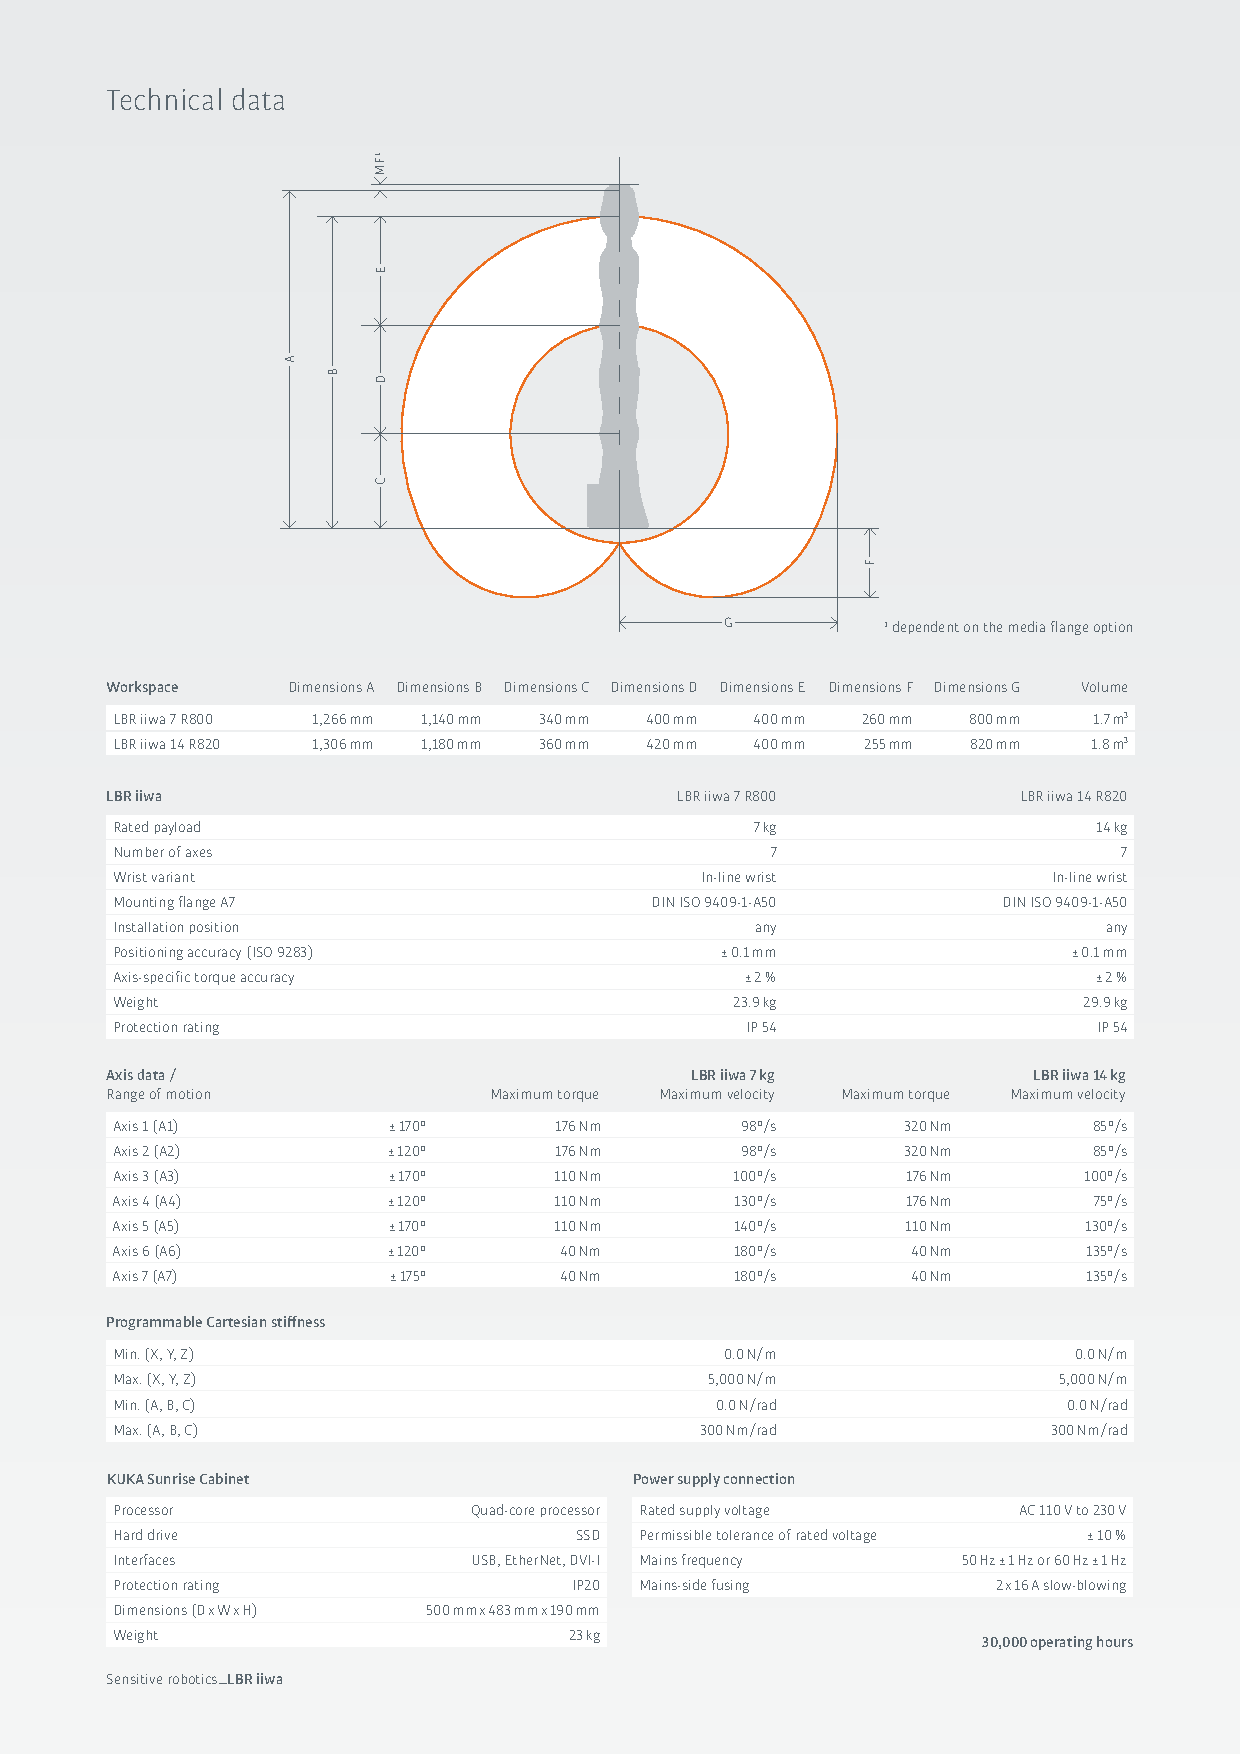
\includegraphics[width=0.95\textwidth]{Imagem/Dim.pdf}
\end{figure}
%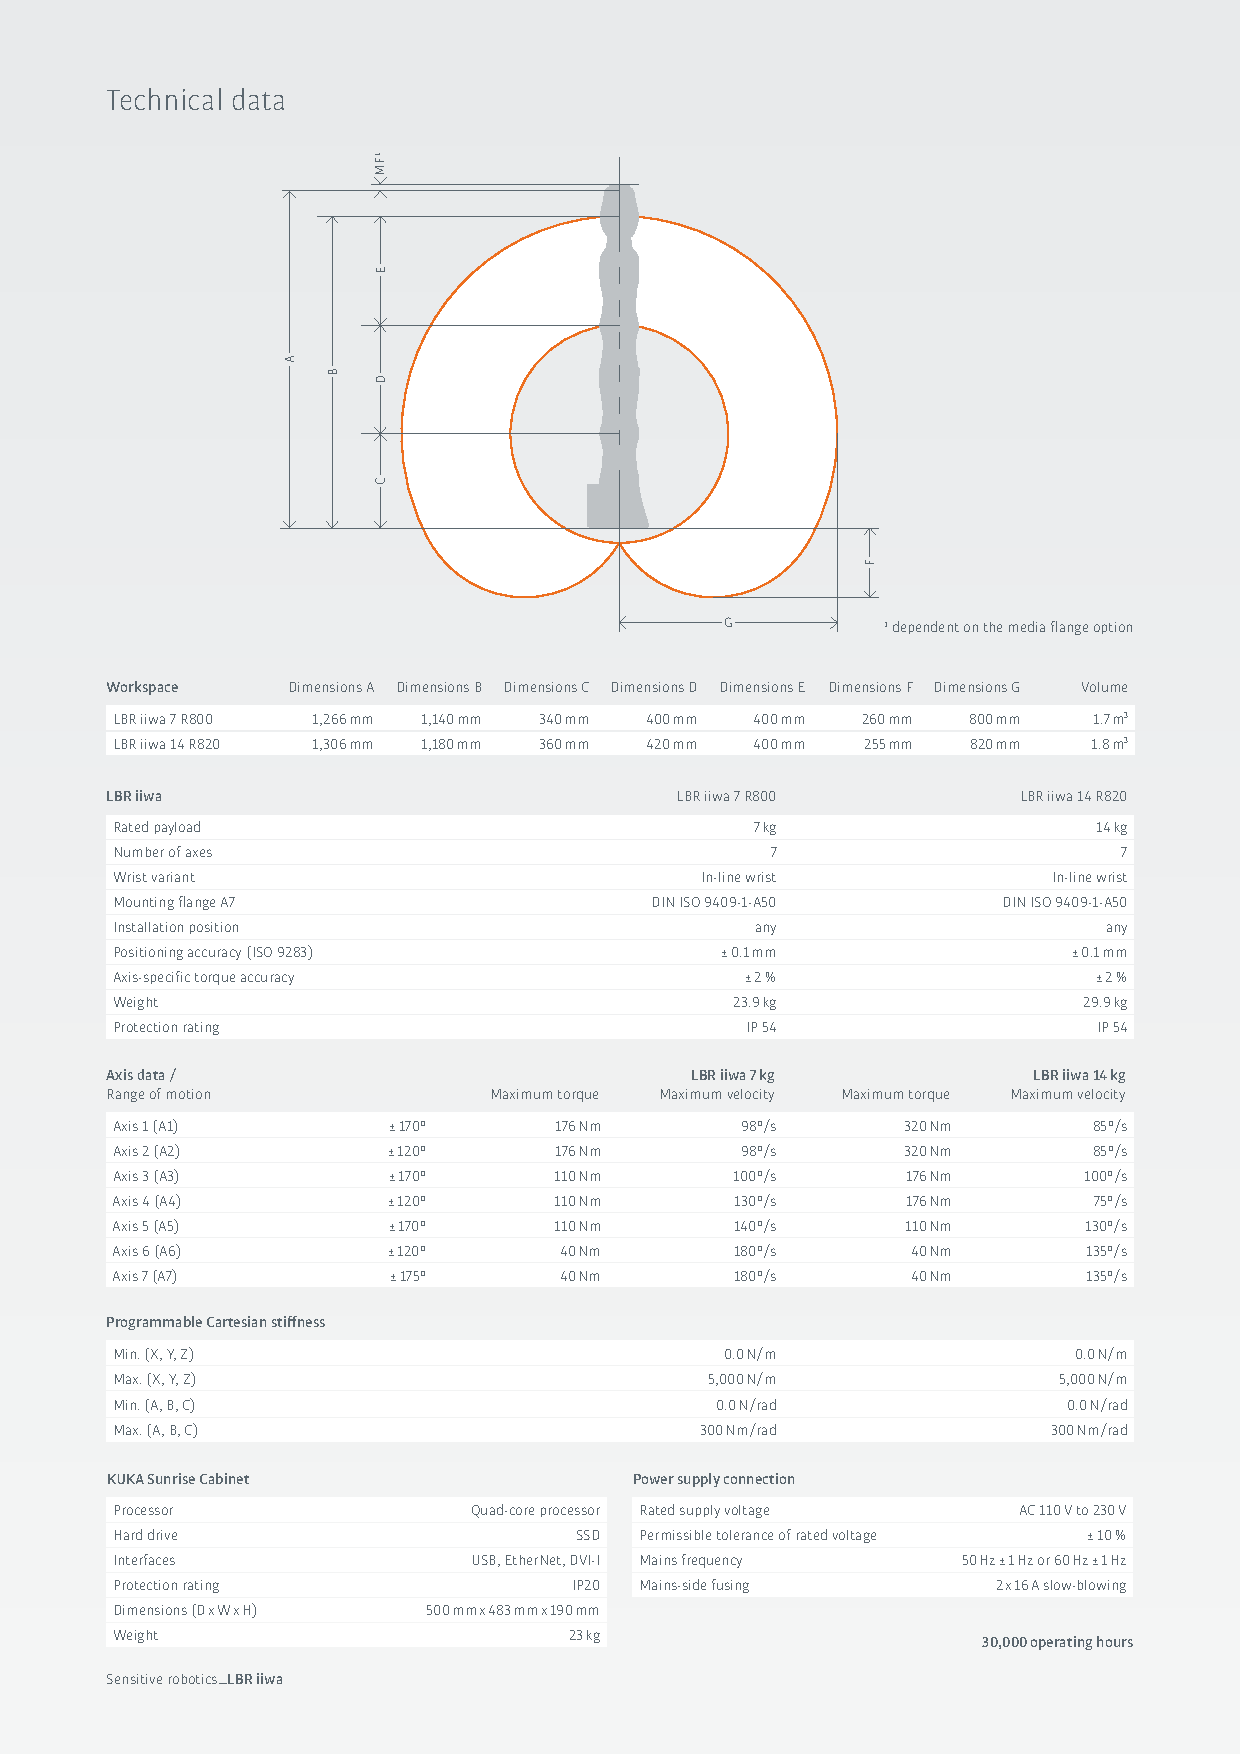
\includepdf[pages=1]{Imagem/Dim.pdf}
\section{Matriz de Transformação \ensuremath{T}}\label{apend:MatrizT}
A multiplicação das matrizes $n$ matrizes de transformação homogênea resulta em
\begin{equation}
    T_{n}^0 = \prod_{i=1}^n A_i = 
    \left[
    \begin{array}{ccc;{2pt/2pt}c}
        r_{11} & r_{12} & r_{13} & d_x \\
        r_{21} & r_{22} & r_{33} & d_y \\
        r_{31} & r_{22} & r_{33} & d_z \\        \hdashline[2pt/2pt]
             0 &      0 &      0 &    1
    \end{array}
    \right]
\end{equation}
na qual os termos são
\begingroup
\footnotesize
\begin{flalign}
    r_{11} =
    \Bigg[\Big[ \left(\left(- s_1 s_3 + c_1 c_2 c_3\right) c_4 + s_2 s_4 c_1\right) c_5 + \left(- s_1 c_3 - s_3 c_1 c_2\right) s_5 \Big] c_6 + 
    \left(\left(- s_1 s_3 + c_1 c_2 c_3\right) s_4 - s_2 c_1 c_4\right) s_6\Bigg] c_7 + \Bigg[- \Big[\left(- s_1 s_3 + c_1 c_2 c_3\right) c_4 \nonumber \\
    %
    %
    + s_2 s_4 c_1\Big] s_5 + \left(- s_1 c_3 - s_3 c_1 c_2\right) c_5\Bigg] s_7 &&
\end{flalign}
\begin{flalign}
    r_{12} = - \Bigg[\Big[\left(\left(- s_1 s_3 + c_1 c_2 c_3\right) c_4 + s_2 s_4 c_1\right) c_5 + \left(- s_1 c_3 - s_3 c_1 c_2\right) s_5\Big] c_6
    + \left(\left(- s_1 s_3 + c_1 c_2 c_3\right) s_4 - s_2 c_1 c_4\right) s_6\Bigg] s_7 + \Bigg[- \Big[\left(- s_1 s_3 + c_1 c_2 c_3\right) c_4 \nonumber \\
    %%
    %%
    + s_2 s_4 c_1\Big] s_5 + \left(- s_1 c_3 - s_3 c_1 c_2\right) c_5\Bigg] c_7 &&
\end{flalign}
\begin{flalign}
r_{13} = 
\Big[\left(\left(- s_1 s_3 + c_1 c_2 c_3\right) c_4 + s_2 s_4 c_1\right) c_5 + \left(- s_1 c_3 - s_3 c_1 c_2\right) s_5\Big] s_6 
- \left(\left(- s_1 s_3 + c_1 c_2 c_3\right) s_4 - s_2 c_1 c_4\right) c_6 &&
\end{flalign}
\begin{flalign}
    r_{21} = \Bigg[\Big[\left(\left(s_1 c_2 c_3 + s_3 c_1\right) c_4 + s_1 s_2 s_4\right) c_5 + \left(- s_1 s_3 c_2 + c_1 c_3\right) s_5\Big] c_6
    + \left(\left(s_1 c_2 c_3 + s_3 c_1\right) s_4 - s_1 s_2 c_4\right) s_6\Bigg] c_7 + \Bigg[- \Big[\left(s_1 c_2 c_3 + s_3 c_1\right) c_4 \nonumber \\
    %%
    %%
    + s_1 s_2 s_4\Big] s_5 + \left(- s_1 s_3 c_2 + c_1 c_3\right) c_5\Bigg] s_7 &&
\end{flalign}
\begin{flalign}
    r_{22} = - \Bigg[\Big[\left(\left(s_1 c_2 c_3 + s_3 c_1\right) c_4 + s_1 s_2 s_4\right) c_5 + \left(- s_1 s_3 c_2 + c_1 c_3\right) s_5\Big] c_6
    + \left(\left(s_1 c_2 c_3 + s_3 c_1\right) s_4 - s_1 s_2 c_4\right) s_6\Bigg] s_7 + \Bigg[- \Big[\left(s_1 c_2 c_3 + s_3 c_1\right) c_4 \nonumber \\
    %%
    %%
    + s_1 s_2 s_4\Big] s_5 + \left(- s_1 s_3 c_2 + c_1 c_3\right) c_5 \Bigg] c_7 &&
\end{flalign}
\begin{flalign}
    r_{23} = 
    \Bigg[\Big[\left(s_1 c_2 c_3 + s_3 c_1\right) c_4 + s_1 s_2 s_4\Big] c_5 + \left(- s_1 s_3 c_2 + c_1 c_3\right) s_5\Bigg] s_6
    - \Big[\left(s_1 c_2 c_3 + s_3 c_1\right) s_4 - s_1 s_2 c_4\Big] c_6 &&
\end{flalign}
\begin{flalign}
r_{31} =
    \Big[\left(\left(- s_2 c_3 c_4 + s_4 c_2\right) c_5 + s_2 s_3 s_5\right) c_6 + \left(- s_2 s_4 c_3 - c_2 c_4\right) s_6\Big] c_7
    + \Big[- \left(- s_2 c_3 c_4 + s_4 c_2\right) s_5 + s_2 s_3 c_5\Big] s_7 &&
\end{flalign}
\begin{flalign}
r_{32} =
    - \Big[\left(\left(- s_2 c_3 c_4 + s_4 c_2\right) c_5 + s_2 s_3 s_5\right) c_6 + \left(- s_2 s_4 c_3 - c_2 c_4\right) s_6\Big] s_7
    + \Big[- \left(- s_2 c_3 c_4 + s_4 c_2\right) s_5 + s_2 s_3 c_5\Big] c_7 &&
\end{flalign}
\begin{flalign}
r_{33} =
    \Big[ \left(- s_2 c_3 c_4 + s_4 c_2\right) c_5 + s_2 s_3 s_5\Big] s_6 - \left(- s_2 s_4 c_3 - c_2 c_4\right) c_6 &&
\end{flalign}
    \begin{flalign}
    d_{x} = 90 \Big[\left(\left(- s_1 s_3 + c_1 c_2 c_3\right) c_4 + s_2 s_4 c_1\right) c_5 + \left(- s_1 c_3 - s_3 c_1 c_2\right) s_5\Big] s_6
    - 90 \Big[\left(- s_1 s_3 + c_1 c_2 c_3\right) s_4 - s_2 c_1 c_4\Big] c_6 - 400 \left(- s_1 s_3 + c_1 c_2 c_3\right) s_4 \nonumber \\
    %%
    %%
    +400 s_2 c_1 c_4 + 420 s_2 c_1 &&
\end{flalign}
\begin{flalign}
    d_y =
    90 \Big[\left(\left(s_1 c_2 c_3 + s_3 c_1\right) c_4 + s_1 s_2 s_4\right) c_5 + \left(- s_1 s_3 c_2 + c_1 c_3\right) s_5 \Big] s_6
    - 90 \Big[\left(s_1 c_2 c_3 + s_3 c_1\right) s_4 - s_1 s_2 c_4\Big] c_6 - 400 \left(s_1 c_2 c_3 + s_3 c_1\right) s_4 \nonumber \\
    + 400 s_1 s_2 c_4 + 420 s_1 s_2 &&
\end{flalign}
\begin{flalign}
    d_z = 90 \Big[\left(- s_2 c_3 c_4 + s_4 c_2\right) c_5 + s_2 s_3 s_5\Big] s_6 - 90 \left(- s_2 s_4 c_3 - c_2 c_4\right) c_6
    + 400 s_2 s_4 c_3 + 400 c_2 c_4 + 420 c_2 + 360 &&
\end{flalign}

\endgroup


\newpage
\section{Memória de cálculo}\label{apend:memoria_calculo}
A memória de cálculo foi realizava via código em \texttt{Python 3}, usando
\begin{mintedbox}{python}
import sympy as sp    # Pacote para manipulaçoes simbolicas
from sympy import pi, cos, sin
from sympy.physics.vector import init_vprinting   # Usada para printar em latex
from sympy.physics.mechanics import dynamicsymbols

init_vprinting(use_latex='mathjax', pretty_print=False)   # Configurando o vprinting

# Variáveis simbólicas
theta1, theta2, theta3, theta4 = dynamicsymbols('theta1 theta2 theta3 theta4')
theta5, theta6, theta7 = dynamicsymbols('theta5 theta6 theta7')
l1, l2, theta, alpha, a, d = dynamicsymbols('l1 l2 theta alpha a d')

# Valores das distancias
dbs, dse, dew, dwf = 360, 420, 400, 90

# Matriz DH:        alfi, ai,  di,  theta
TDH = sp.Matrix([ [-pi/2,  0, dbs, theta1],
                  [ pi/2,  0,   0, theta2],
                  [ pi/2,  0, dse, theta3],
                  [-pi/2,  0,   0, theta4],
                  [-pi/2,  0, dew, theta5],
                  [ pi/2,  0,   0, theta6],
                  [    0,  0, dwf, theta7]])

# Rotação de theta em z com Rotação de alpha em x
Rot = sp.Matrix([[cos(theta), -sin(theta)*cos(alpha),  sin(theta)*sin(alpha)],
                 [sin(theta),  cos(theta)*cos(alpha), -cos(theta)*sin(alpha)],
                 [         0,             sin(alpha),             cos(alpha)]])

# Translação dos links
Tran = sp.Matrix([a*cos(theta),a*sin(theta),d])
# Distorção e Escala
S = sp.Matrix([[0, 0, 0, 1]])

# Matriz A genérica
A = sp.Matrix.vstack(sp.Matrix.hstack(Rot, Tran), S)


# Matriz A de cada linha
A1 = A.subs({ alpha:TDH[0,0], a:TDH[0,1], d:TDH[0,2], theta:TDH[0,3] })
A2 = A.subs({ alpha:TDH[1,0], a:TDH[1,1], d:TDH[1,2], theta:TDH[1,3] })
A3 = A.subs({ alpha:TDH[2,0], a:TDH[2,1], d:TDH[2,2], theta:TDH[2,3] })
A4 = A.subs({ alpha:TDH[3,0], a:TDH[3,1], d:TDH[3,2], theta:TDH[3,3] })
A5 = A.subs({ alpha:TDH[4,0], a:TDH[4,1], d:TDH[4,2], theta:TDH[4,3] })
A6 = A.subs({ alpha:TDH[5,0], a:TDH[5,1], d:TDH[5,2], theta:TDH[5,3] })
A7 = A.subs({ alpha:TDH[6,0], a:TDH[6,1], d:TDH[6,2], theta:TDH[6,3] })

# Matriz de transformação de 7 (end-effector) para 0
T = A1*A2*A3*A4*A5*A6*A7

# Validação: home (todas as juntas em 0)
Thome = T.subs({ theta1:0, theta2:0, theta3:0, theta4:0, theta5:0, theta6:0, theta7:0 })

# Validação: posição qualquer (comparar o resultado com a interpretação física)
q1, q2, q3, q4, q5, q6, q7 = 0, 0, 0, -pi/2, pi/3, 0, 0
T_ = T.subs({ theta1:q1, theta2:q2, theta3:q3, theta4:q4, theta5:q5, theta6:q6, theta7:q7 })

\end{mintedbox}

\end{document}
